
\documentclass[preprint,12pt,authoryear]{elsarticle}

\usepackage{graphicx} % Required for inserting images
\usepackage{titlesec}
\usepackage{float}
\usepackage{graphicx}
\usepackage{amsmath}
\usepackage{amssymb}
\usepackage{mathpazo}
\usepackage{datetime}
\usepackage{hyperref}
\usepackage{bookmark}
\usepackage{mathtools}
\usepackage{caption}
\usepackage{subcaption}
\usepackage{hyperref} % Add this package to use hyperlinks
\usepackage{colortbl}
\usepackage{longtable}
\usepackage{booktabs} % For \toprule, \midrule, \bottomrule
\usepackage{lineno}
\linenumbers
\usepackage{multirow}
\usepackage{enumitem}
\usepackage[normalem]{ulem}
\usepackage{booktabs, multirow, xcolor, colortbl}

\usepackage{algorithmic}
% \usepackage[longnamesfirst,square,numbers,comma,sort&compress]{natbib}
\usepackage{tabularx}
\usepackage{array}
\usepackage{tabularx}
\usepackage{booktabs}
\usepackage{array}
\usepackage{xcolor}
\usepackage{pdflscape}
\usepackage{pifont}
\usepackage{mdframed}
\usepackage{rotating}
\usepackage{geometry}
\geometry{a4paper, margin=1in}
\usepackage{lscape}
\usepackage{afterpage}
\newcommand{\cmark}{\ding{51}} % Define command to print check mark
\newcommand{\xmark}{\ding{55}} % Define command to print x mark
\usepackage{pifont}
\usepackage{booktabs, multirow, xcolor}

\usepackage{booktabs}
\usepackage{arydshln} % for dashed lines
\usepackage[table]{xcolor} % for coloring cells


\usepackage{booktabs,colortbl,xcolor}
\definecolor{HardCol}{RGB}{220,  50, 47}    % red  
\definecolor{MedCol} {RGB}{255,165,  0}    % orange  
\definecolor{EasyCol}{RGB}{ 38,155, 36}    % green  
\definecolor{FragCol}{RGB}{150,150,150}    % gray




% Define new column types for uniform styling and functionality
\newcolumntype{M}[1]{>{\centering\arraybackslash\small}m{#1}} % Small font, centered
\newcolumntype{B}[1]{>{\centering\arraybackslash\small\bfseries}m{#1}} % Bold font, centered
\newcolumntype{S}{>{\centering\arraybackslash\small\bfseries}m{0.8cm}} % Small and bold font, fixed width
\newcolumntype{T}{>{\centering\arraybackslash\tiny\bfseries}m{0.8cm}} % Small and bold font, fixed width

\usepackage{algpseudocode}
\usepackage{booktabs}
\usepackage{longtable} % Add this package for long tables that split over pages
\usepackage{graphicx}  % Needed for \resizebox
\usepackage{pgfplots}


%% The amssymb package provides various useful mathematical symbols
\usepackage{amssymb}
%% The amsmath package provides various useful equation environments.
\usepackage{amsmath}
%% The amsthm package provides extended theorem environments
%% \usepackage{amsthm}

%% The lineno packages adds line numbers. Start line numbering with
%% \begin{linenumbers}, end it with \end{linenumbers}. Or switch it on
%% for the whole article with \linenumbers.
%% \usepackage{lineno}

\journal{Knowledge Based Systems}

\begin{document}

\begin{frontmatter}
    \title{Choosing the Right Dataset: Hardness Criteria for Feature Selection Benchmarking}

\author[aff1]{Itamar Elmakias}
\ead{itamare@post.bgu.ac.il}

\author[aff1]{Dan Vilenchik}
\ead{vilenchi@bgu.ac.il, corresponding author}

\affiliation[aff1]{organization={School of Electrical and Computer Engineering, Ben-Gurion University of the Negev},%Department and Organization
            addressline={POB 653}, 
            city={Beer-Sheva},
            postcode={8410501}, 
            country={Israel}}


%% Abstract
\begin{abstract}
%% Text of abstract

Feature selection (FS) is a core component of many machine learning pipelines, with numerous algorithms already proposed and new ones continually emerging. Yet the benchmarking process—both for existing methods and those to come—suffers from a key limitation: widely used datasets are rarely ranked by difficulty, and there is no canonical set of ‘hard’ datasets against which meaningful progress can be demonstrated. To address this gap, we introduce a principled, data-driven framework for categorizing dataset difficulty into three levels—Easy, Medium, and Hard—based on the utility gained from applying FS. Our empirical analysis spans 63 binary and 39 multi-class popular datasets and 27 FS algorithms. While no dataset met the ‘Hard’ threshold, 11 were identified as ‘Medium’. We further propose a peeling procedure that transforms datasets into more challenging variants while preserving ground-truth features—a valuable benchmark property. This yielded two  'Hard' datasets, resulting in a curated suite of 13 challenging benchmarks for FS evaluation. All data and tools are publicly available to support ongoing, community-driven benchmarking.


\end{abstract}

% %%Graphical abstract
% \begin{graphicalabstract}
% %\includegraphics{grabs}
% \end{graphicalabstract}

% %%Research highlights
\begin{highlights}
\item We introduce a framework for discrete categorization of dataset complexity to be used in benchmarking feature selection algorithms.
\item An extensive analysis of 102 popular datasets shows that the majority are not inherently challenging.
\item We propose a peeling procedure to generate hard datasets while preserving ground truth.
\item We offer an end-to-end platform where researchers can upload their datasets or feature selection algorithms into a shared evaluation queue and receive profiling results. Uploaded datasets are evaluated across 27 feature selection algorithms, and new algorithms are benchmarked against 102 pre-profiled datasets with established performance baselines.



\end{highlights}

%% Keywords
\begin{keyword}
 Feature selection \sep Curse of dimensionality \sep Machine learning benchmarks \sep High-dimensional data \sep Dataset complexity \sep Explainable AI \sep Dimensionality reduction

%% MSC codes
\MSC[2020] 62R07 \sep 68T09 \sep 62P99 \sep 68W40 \sep 62H99
\end{keyword}


\end{frontmatter}

%% Add \usepackage{lineno} before \begin{document} and uncomment 
%% following line to enable line numbers
%% \linenumbers

%% main text
%%

%% Use \section commands to start a section
\section{Introduction}




\label{chapter:intro}
Feature selection (FS) is a foundational task in machine learning, used to reduce dimensionality, improve model performance, and enhance interpretability. By identifying and retaining only the most informative features, FS helps address challenges such as overfitting, noise sensitivity, and computational inefficiency. FS is especially needed in settings where the number of features far exceeds the number of samples—a situation often described as high-dimensional (HD) data. 


The abundance of FS algorithms reflects the absence of a universal ``best" method for all tasks. Numerous surveys, e.g., \citep{weston2000feature, guyon2003introduction, chandrashekar2014survey, bolon2014review, li2017feature, bommert2020benchmark, bommert2022benchmark, jiao2023survey}, compare and benchmark different FS methods, many of which focus on high-dimensional data. A typical FS paper or survey follows a common structure: a subset of FS algorithms is selected (typically no more than 20), along with a subset of datasets for benchmarking (again, usually no more than 20). While there is sometimes a rationale behind the choice of algorithms (more in survey papers than in method papers)—such as evaluating univariate vs. multivariate methods or supervised vs. unsupervised approaches—there is rarely a clear explanation for the specific choice of datasets. When a justification is provided, it is often based on general criteria, such as the dataset’s popularity in prior studies or its high dimensionality. This lack of a systematic approach to dataset selection limits the generality and strength of conclusions drawn from such studies. Table \ref{tab:survey_papers} summarizes the number of datasets and algorithms used in highly cited FS survey papers. The papers in Table  \ref{tab:survey_papers} were selected by performing a Google Scholar search for “feature selection survey” and randomly picking several top-cited papers from the first page of results. 


\begin{table}[h!]
\centering \caption{Summary statistics for prominent FS survey papers. Papers are sorted by number of citations. The table shows the typically limited number of datasets and algorithms that were surveyed.}{\small
\begin{tabularx}{0.7\textwidth}{|>{\centering\arraybackslash}X|>{\centering\arraybackslash}X|>{\centering\arraybackslash}X|>{\centering\arraybackslash}X|} % Adjusts table to 70% of text width and centers the text
\hline
\textbf{Paper, Year} & \textbf{\#Citations} & \textbf{\# Datasets} & \textbf{\# Algorithms} \\
\hline
\citep{chandrashekar2014survey}, 2014 & 5728 & 7 & 2 \\
\hline
\citep{li2017feature}, 2017 & 3353 & 29 & 34 \\
\hline
\citep{bolon2014review}, 2014 & 756 & 9 & 7 \\
\hline
\citep{zhang2019unsupervised}, 2019 & 126 & 16 & 8 \\
\hline
\citep{bommert2020benchmark}, 2020 & 636 & 16 & 22 \\
\hline
\citep{bommert2022benchmark}, 2022 & 107 & 14 & 11 \\
\hline
\citep{tanveer2022large}, 2022 & 38 & 14 & 11 \\
\hline
\citep{jiao2023survey}, 2023 & 57 & 2 & 23 \\
\hline
\end{tabularx}}


\label{tab:survey_papers}
\end{table}

Another consideration in evaluating FS algorithms is the common reliance on incremental performance comparisons, which, while precise, may limit broader insights. For example, many studies compare two FS pipelines \(P_1\) and \(P_2\) on a dataset \(D\) by reporting results such as: “The accuracy after applying feature selection with \(P_1\) was \(78\%\), compared to \(81\%\) with \(P_2\), showing a \(3\%\) improvement.” While such comparisons are useful for measuring gains, they may not always provide a clear understanding of broader trends across datasets or algorithms, particularly when performance is highly dataset-specific. Even with statistical significance testing, granular analyses can struggle to offer a conceptual view of FS algorithm effectiveness.

We do not suggest replacing incremental evaluations—on the contrary, they remain essential. Rather, they can be complemented by higher-level abstractions. One useful addition is a categorical framework that assigns performance to discrete levels—such as High, Fair, and Low—based on well-established cut-offs. 

The two gaps we identified—namely, the absence of a principled approach to dataset selection and the focus on incremental performance improvements—are closely related. When evaluation is centered primarily on performance gains, it becomes difficult to develop a broader perspective on the relative difficulty of datasets. This, in turn, limits the ability to establish a clear rationale for selecting datasets for benchmarking.

To address these intertwined issues, we propose a unified framework grounded in discrete performance categories. Building upon these categories, we introduce a new method for classifying datasets by hardness and use it to rank 102 popular datasets that are used in the FS literature. This repository may serve as a foundation for evaluating new FS algorithms or conducting comparative studies.


The key challenge in defining our framework lies in delineating clear category boundaries. A foundational line of work on dataset complexity \citep{ho2002complexity} proposed twelve quantitative measures to capture the intrinsic difficulty of classification problems—such as class overlap, feature-to-sample ratio, linear separability, and neighborhood consistency. These measures were later expanded to twenty-two and made publicly available through the \href{https://github.com/w4k2/problexity?utm_source=chatgpt.com}{\texttt{problexity}} repository \citep{problexity}, with a comprehensive review provided by \citet{lorena2019complexity}. Notably, Ho and Basu did not define a ground truth for dataset hardness or rank datasets by difficulty; their analysis was exploratory. Subsequent studies applied their framework to real-world datasets, computing similar metrics and validating them empirically against what they treated as the ground truth for hardness—the observed \emph{classifier performance} \citep{lorena2012complex,kamath2008structured,garcia2016multiple,moran2017data}. 

The Ho and Basu framework was designed as a \emph{prospective} tool to predict which datasets are likely to be hard for classification before training. In contrast, our study takes a \emph{retrospective} perspective: we examine the datasets that are already widely used to benchmark FS algorithms and ask whether these benchmarks are indeed challenging in practice. To this end, we adapt the Ho and Basu paradigm to suit retrospective analysis. We first identify ``Easy'' datasets empirically: informally, if running an off-the-shelf tabular learner such as a Random Forest or a boosted model yields high performance (e.g., AUC or accuracy above $90\%$), the dataset can be considered trivially easy, and no further analysis is needed. For datasets where performance is lower, several explanations are possible---the model or its parameters may be suboptimal, or the dataset may indeed be intrinsically more complex. While our exhaustive set of FS algorithms helps mitigate the first concern, we further draw on the Ho and Basu framework to provide a more theoretically grounded interpretation. Specifically, we compare the observed low-performing datasets against the ``Easy'' ones (for which difficulty is known a posteriori) and assess whether the data-centric hardness indicators align with the empirically observed performance. Combining empirical evidence with these established complexity measures yields a robust and interpretable criterion for identifying challenging benchmark datasets for FS research.



Still, several practical choices remain to be made in translating this general perspective into an operational framework for feature selection benchmarking. For example, a dataset might be considered 'Hard' if ML pipelines applied to it, as reported in the literature, perform poorly (e.g., achieving accuracy barely above guessing the majority class). Alternatively, a dataset could be labeled 'Hard' if, regardless of the feature selection method applied, the resulting ML pipeline performance shows minimal improvement or even deteriorates. In Section~\ref{sec:methodology}, we offer a rigorous definition of the hardness categories, but for now, we proceed with the intuitive understanding of hardness outlined here.


The first step in curating a database of categorized datasets is collecting popular datasets, those that are frequently used in the evaluation of FS algorithms and are publicly available through open repositories. These datasets constitute the de facto standard for empirical validation in the FS community, and are thus directly relevant to how new methods are developed, tuned, and compared. We acknowledge that this introduces a potential bias: challenging datasets that researchers have encountered but chosen not to publish—perhaps due to poor results—are unlikely to be represented. Nevertheless, our goal is not to claim completeness, but to reflect the current state of FS evaluation practice. 


Before presenting our contributions, we conclude with two remarks to further contextualize our results. 

(1) Generating \emph{synthetic} datasets with controllable difficulty is a well-established practice, typically done by adjusting parameters such as the signal-to-noise ratio or introducing noise to weaken correlations between features and targets. Statistical generative models like the Single-Spike Sparse-PCA offer control over problem difficulty and have led to important insights about feature recovery \cite{RigolletAOS,johnstone2009consistency,Wainwright06,AminiWain09}. Also, the work of \cite{ho2002complexity} used a synthetic dataset (alongside real-world) for their study.
 \cite{bolon2013review} wrote a survey on evaluating FS methods on synthetic benchmarks.

However, such theoretical models rarely trickle down to practice. Many feature selection studies rely on real-world datasets that are noisy, heterogeneous, and not constructed with known hardness guarantees. Our focus in this paper is on evaluating these commonly used datasets systematically. Building a theoretical foundation to explain their hardness would be a valuable contribution; our work here may provide the empirical groundwork for such efforts. 


(2) Performance alone does not capture all aspects of dataset complexity. Structural properties such as feature redundancy, higher-order interactions, robustness, and alignment with domain knowledge can indeed influence dataset complexity. However, some of these objectives are often more reflective of FS algorithm behavior than of the datasets themselves. We aim to separate the algorithmic component (how FS methods operate) from the evaluation language (how datasets respond).

Furthermore, performance is the primary metric reported in papers introducing new FS algorithms. To align with this norm and support broad adoption, we focus on performance-based evaluation. In the trade-off between detail and clarity, we opt for a simple benchmarking scaffold, leaving multi-objective analysis for future work.



\paragraph{{\bf Our Contribution.}}
The aforementioned issues reveal a methodological gap: the FS community lacks clear criteria for dataset difficulty and relies on benchmarks that may be too easy. We address this by quantifying the problem and proposing a more principled evaluation framework.


\vspace{1mm}


We begin by introducing an empirically grounded measure of dataset hardness, based on the utility gained from feature selection. This allows us to categorize datasets into three levels of difficulty—'Easy', 'Medium', and 'Hard'—as detailed in Section~\ref{sec:methodology}. Applying this framework, we analyzed widely-used 63 binary and 39 multi-class datasets using 27 FS algorithms, resulting in over 11,000 experiments.


Our analysis revealed that \emph{none} of the 63 binary datasets qualified as 'Hard'; 11 were labeled 'Medium' and 52 as 'Easy'. In that analysis, we took the average cross-validation performance of the best algorithm as the key to deciding the level of difficulty.  Following the common ML practice of requiring differences larger than one standard deviation to claim significance \cite{kohavi1995study}, 9 of the 11 ‘Medium’ datasets would be reclassified as ‘Hard.’ Notably, these nine are also the noisiest in our collection—measured by cross-validation variance—consistent with prior findings that link noise to dataset hardness.

All datasets and source code for the feature-selection algorithms are publicly available in our GitHub repository.\footnote{\url{https://github.com/Itamarelmakia/FeatureSelect-Benchmark-Hub/tree/main}}


We further validated our performance-based categorization using the twenty-two intrinsic data-complexity indices implemented in the \texttt{problexity} library \cite{problexity}. The empirical differences between the ‘Easy’ and ‘Medium’ datasets aligned with the complexity indices, reinforcing the consistency between observed performance and intrinsic data characteristics.



\vspace{1mm}

To address the scarcity of challenging benchmarks, we developed a controlled peeling procedure designed to create hard datasets from existing data. Our method systematically reduces dataset size while preserving a small, high-performing feature subset (a ground truth). The presence of a ground truth ensures that these datasets are not pathologically hard due to noise or data degradation; rather, they remain genuinely informative yet difficult for existing FS algorithms. 

Applying the peeling procedure across all 102 datasets produced two 'Hard' datasets: the peeled version of Slashdot \cite{read2011classifier} and SMK-CAN-187 \cite{li2017feature}—in which the retained feature subset yielded strong performance, yet none of the 27 tested algorithms succeeded in recovering it or a comparable one. The remaining 100 datasets failed to retain predictive power post-peeling.

The two peeled 'Hard' datasets, together with the 11 'Medium' datasets, offer a set of 13 challenging datasets from which researchers studying FS can choose benchmarks. The 11 'Medium' datasets are: Period Changer~\cite{period_changer_729}, Slashdot~\cite{read2011classifier}, tumors\_C~\cite{read2011classifier}, Breast~\cite{pochet2004systematic},
Hepatitis~\cite{hepatitis_46}, 
CNS~\cite{pomeroy2002prediction}, 
Colon~\cite{alon1999broad}, 
HIVA~\cite{guyon2006performance}, 
SMK-CAN-187~\cite{li2017feature}, Bioresponse~\cite{vanschoren2014openml}, Titanic~\cite{ekinci2018comparative}.
 Among these, the first nine datasets can be considered ‘Hard’ under the one-standard-deviation adjustment, while the latter two remain solidly in the ‘Medium’ category.
\vspace{1mm}

We further introduce a complementary notion of dataset complexity: the 'Fragile' category, which captures cases where applying FS reduces performance enough to downgrade the dataset’s difficulty classification—e.g., from 'Easy' to 'Medium'. We found \emph{no} 'Fragile' datasets among the 102 we analyzed.

\vspace{1mm}

Building on this analysis, we aim to support the FS community through practical tools that lower the barrier to rigorous evaluation. To this end, we are developing an end-to-end platform where researchers will be able to submit their datasets or feature selection algorithms to a shared evaluation queue and receive detailed profiling results. This approach is particularly useful for researchers without the resources to run extensive pipelines—spanning 27 FS algorithms and 102 datasets—locally. 
\vspace{1mm}




Finally, we reflect on our results in light of the well-known curse of dimensionality~\cite{bellman1957dynamic,donoho2000high,RigolletAOS,AminiWain09}, which warns that when features far outnumber samples, FS should become unreliable, leading to overfitting and degraded performance. Across 102 datasets, many labeled as high-dimensional and real-world, we observed only weak adverse effects. More concretely, we computed correlations between class imbalance and performance, as well as between the dimensionality ratio and performance (two widely used dataset complexity indices). Across the 63 binary datasets, we found no significant association in either case. This does not invalidate theoretical concerns, nor imply such challenges never arise, but it does point to a gap between high-dimensional theory and the empirical behavior of real-world data. Part of this may stem from the retrospective nature of our analysis, which focuses on benchmark datasets already established in FS research and thus biased toward tractable problems. In either case, these findings serve as a caution against invoking descriptors such as “high-dimensional” or “imbalanced” as automatic indicators of difficulty, underscoring the need for empirical validation in guiding FS benchmarking.


\vspace{3mm}

The remainder of the paper is organized as follows. In Section \ref{sec:related} we cover related work.  Section~\ref{sec:methodology}, we introduce our framework for categorizing dataset hardness. Section \ref{sec:dataset} provides the details of the 102 datasets that we curated,  and Section~\ref{sec:exp_setting} details our experimental setup, including a full description of the pipeline we've used. In Section~\ref{sec:results}, we present the empirical results of applying our framework to 102 real-world datasets. Section~\ref{sec:peeling} details our peeling procedure for generating hard datasets with a defined ground truth, and Section~\ref{sec:intrinsic} provides a comprehensive account of the dataset complexity indices and their correspondence to the empirical categorization. We conclude with limitations in Section \ref{sec:limit} and discussion in  Section~\ref{sec:discussion} of the implications of our findings for FS research and future directions.





\section{Related Work}\label{sec:related}
Feature selection (FS) is a well-established area in machine learning, with numerous surveys having mapped the landscape of FS algorithms, offering useful taxonomies and practical guidance, \cite{bolon2015recent,li2017feature,theng2024feature,nouri2023novel} to mention just a few. While much effort has gone into developing and comparing FS methods, far less attention has been given to the datasets used for benchmarking. The most closely related work is by Li~\emph{et al.}~\cite{li2017feature}, who survey FS methods by data type. In contrast, we propose dataset \emph{hardness} as a new axis of evaluation to guide principled benchmark design.

For completeness, we briefly review the main FS paradigms—filter, wrapper, embedded, ensemble, and hybrid—and summarize the 27 algorithms used in our study. Full details appear in Table~\ref{tab:FS_algs}. 

\textbf{Filter Methods} evaluate each feature \emph{independently}, without training a predictive model. We adopt the common three-way breakdown:  
(i) \emph{Statistical tests} — Low Variance~\cite{pedregosa2011scikit,johnstone2009consistency}, Skewness~\cite{hochma2024efficient}, UnivariateFS~\cite{pedregosa2011scikit}, Leading Eigenvector (LeadingEV)~\cite{d2004direct}, and Covariance Thresholding (CT)~\cite{Bickel2008CovarianceMatrices};  
(ii) \emph{Information-theoretic criteria} — Minimum Redundancy Maximum Relevance (mRMR)~\cite{peng2005feature}, and ReliefF~\cite{robnik2003theoretical};  
(iii) \emph{Geometry-based scores} — Laplacian Score (LS)~\cite{he2005laplacian} and Multi-Cluster Feature Selection (MCFS)~\cite{cai2010unsupervised}.  
%These methods serve as fast, model-agnostic baselines before turning to more computationally intensive wrappers, embedded methods, or hybrids.
{\small
\begin{table}[t!]
\centering
\caption{Summary of the 27 feature-selection algorithms used. Category: Filter (F), Wrapper (W), Embedded (E), Ensemble-embedded (En), Hybrid (H).}
\resizebox{\textwidth}{!}{
\begin{tabular}{|c|l|c|c|c|c|c|c|}
\hline
\textbf{\#} & \textbf{Algorithm} & \textbf{Year} & \textbf{\# Citations} & \textbf{Supervised} & \textbf{Hyperparams} & \textbf{Category} & \textbf{Source} \\
\hline
1  & DecisionT\_B \cite{guyon2003introduction}           & 2003 & 21344 & \checkmark & \checkmark & W   & GitHub \\
2  & DecisionT\_F \cite{guyon2003introduction}           & 2003 & 21344 & \checkmark & \checkmark & W   & GitHub \\
3  & ReliefF \cite{kira1992feature}                      & 2003 & 3785  & \checkmark & \checkmark & F   & GitHub \\
4  & SVM\_B \cite{guyon2003introduction}                 & 2003 & 21344 & \checkmark & \checkmark & W   & GitHub \\
5  & SVM\_F \cite{guyon2003introduction}                 & 2003 & 21344 & \checkmark & \checkmark & W   & GitHub \\
6  & LeadingEV \cite{d2004direct}                        & 2004 & 1251  & \checkmark & \checkmark & F   & in-house \\
7  & Alpha Inv \cite{zhou2005streaming}                  & 2005 & 122   & \checkmark & \checkmark & W   & GitHub \\
8  & LS \cite{he2005laplacian}                           & 2005 & 2781  & X          & \checkmark & F   & GitHub \\
9  & mRMR \cite{peng2005feature}                         & 2005 & 11965 & \checkmark & \checkmark & F   & GitHub \\
10 & ETree \cite{geurts2006extremely}                    & 2006 & 8620  & \checkmark & \checkmark & En  & scikit-learn \\
11 & CT \cite{Bickel2008CovarianceMatrices}                               & 2008 & 1587  & X          & X          & F   & in-house \\
12 & AdaBoost \cite{hastie2009multi}                     & 2009 & 2520  & \checkmark & \checkmark & En  & scikit-learn \\
13 & DT (Diagonal Thr.) \cite{johnstone2009consistency}  & 2009 & 1010  & X          & X          & F   & in-house \\
14 & MCFS \cite{cai2010unsupervised}                     & 2010 & 1352  & X          & X          & E   & GitHub \\
15 & RFS \cite{nie2010efficient}                         & 2010 & 2492  & \checkmark & \checkmark & E   & GitHub \\
16 & SVM RBF \cite{liu2011feature}                       & 2011 & 130   & \checkmark & \checkmark & E   & scikit-learn \\
17 & Low Var \cite{pedregosa2011scikit}                  & 2011 & 99602 & X          & X          & F   & GitHub \\
18 & UnivariateFS \cite{pedregosa2011scikit}             & 2011 & 99602 & \checkmark & \checkmark & F   & scikit-learn \\
19 & GRAPH \cite{ye2012sparse}                           & 2012 & 113   & \checkmark & \checkmark & E   & GitHub \\
20 & SVC \cite{abraham2014machine}                       & 2014 & 1988  & \checkmark & \checkmark & E   & scikit-learn \\
21 & CAE \cite{balin2019concrete}                        & 2019 & 164   & X          & \checkmark & E   & GitHub \\
22 & DLFS \cite{wojtas2020feature}                       & 2020 & 152   & \checkmark & \checkmark & E   & GitHub \\
23 & UFS \cite{cheng2021algorithmic}                     & 2021 & 9     & X          & \checkmark & E   & GitHub \\
24 & SHAP \cite{lundberg2017unified}                     & 2017 & 34948 & \checkmark & \checkmark & E   & scikit-learn \\
25 & GRACES \cite{chen2023graph}                         & 2023 & 12    & \checkmark & \checkmark & E   & GitHub \\
26 & Skewness \cite{hochma2024efficient}                 & 2024 & 1     & X          & X          & F   & scipy \\
27 & CEI\_GA \cite{nematzadeh2024feature}                & 2024 & 4     & \checkmark & \checkmark & H   & GitHub \\
\hline
\end{tabular}}
\label{tab:FS_algs}
\end{table}
}




\textbf{Wrapper Methods} embed a predictive model inside a search procedure: a candidate subset is evaluated by training the model, a score (e.g.\ accuracy or AUC) is recorded, and the search continues until a stopping rule is met.  Typical search strategies include greedy stepwise selection and recursive feature elimination (RFE).  Wrappers often yield high-quality subsets but are computationally expensive.  In this work, we use the classical stepwise RFE variants—DecisionTree\_Forward (and the backward version), SVM\_Forward (and backward) \cite{guyon2003introduction}—together with the online Alpha Investing wrapper \cite{zhou2005streaming}, which sequentially tests incoming features under a controlled false-discovery budget.


\textbf{Embedded Methods} select features \emph{within} a model’s own learning objective, so no external search loop is required.  
We ran methods from different sub-families of wrapper methods, including: (i) \emph{Sparsity-penalised linear models}—RFS\,\cite{nie2010efficient} represents the family of LASSO/Elastic-Net style methods that shrink irrelevant coefficients to zero;  
 (ii) \emph{Graph-regularised selectors}—Graph Lasso (GRAPH)\,\cite{ye2012sparse} enforces smoothness on a feature-affinity graph, a strategy highlighted in modern reviews of structure-preserving FS; (iii) \emph{NN-based (deep) selectors}—Concrete Auto-Encoder (CAE)\,\cite{balin2019concrete}, DLFS\,\cite{wojtas2020feature}, the graph-CNN selector GRACES\,\cite{chen2023graph}, and the unsupervised UFS\,\cite{cheng2021algorithmic} learn differentiable masks during network training;   (iv) \emph{Model-driven importance} — we include the permutation-importance SVM\_RBF selector \cite{liu2011feature} and
SHAP~\cite{lundberg2017unified}, which ranks features by their absolute Shapley value contributions computed on a trained gradient-boosted tree ensemble.
%, in line with the “model-driven importance” sub-family discussed by Moslemi \cite{moslemi2023tutorial}.  

% Because feature importance is optimized jointly with model fitting, embedded methods deliver near-wrapper accuracy while retaining filter-level efficiency.

\textbf{Ensemble Methods} are an embedded subclass that \emph{aggregate} importance scores from many weak learners.  
We employ ExtraTrees (ETree)\,\cite{geurts2006extremely} and AdaBoost-SAMME (AdaBoost)\,\cite{hastie2009multi}.%: each tree or stump contributes votes based on impurity reduction, and the aggregation yields a stable, low-variance ranking—particularly valuable for high-dimensional or noisy data.

\textbf{Hybrid Methods} combine the speed of a filter with the thoroughness of a wrapper or embedded selector in a two-stage pipeline.  
In this study, we use CEI\_GA\cite{nematzadeh2024feature}, which first screens features with Classification Error Impurity (CEI) and then refines the top-ranked candidates via a genetic-algorithm wrapper. % This cascade preserves filter efficiency—by discarding obviously irrelevant variables early—while allowing the wrapper to explore high-quality subsets within the reduced search space.


\section{Methodology}\label{sec:methodology}
In this section, we present our methodology to categorize the hardness of a dataset. The methodology hinges upon two choices: what ML pipeline to run and which FS algorithms to use. In Section~\ref{sec:exp_setting}, we elaborate on the choice and parametrization of both the ML and FS pipelines, including the choice of $k$ (the size of the feature set); we defer these implementation details to avoid interrupting the conceptual flow of the methodology presented here.

The category is derived from two quantities:
\begin{itemize}
    \item{\bf{Q1}} \emph{ What performance can be achieved by running a suitable ML pipeline without FS?} We measure performance, over a stratified 5-CV test, using standard measurements (specifically, accuracy and AUC). 
    
    \item{\bf{Q2}} \emph{What performance can be achieved by running FS before the ML pipeline?}  
    To answer this, a suite of FS algorithms is applied with different values of \(k\) (the number of selected features). The ML pipeline is then used to evaluate performance after reducing the dataset to the selected features. As part of the evaluation process, a stratified 5-CV is employed, where FS is performed on the training set, and performance is measured on the test set (as the average of the five folds). Figure \ref{fig:method_pipeline} provides a visual representation of this methodology.

    To answer Q2, we take the maximum performance across all executions (across all FS algorithms and \(k\) values). This adversarial choice is logically justified in the context of identifying 'Hard' datasets, as it represents the most conservative quantifier. By taking the maximum performance, we ensure that even under the most favorable conditions, if a dataset's performance remains poor, it is genuinely 'Hard.'   In Sections~\ref{sec:ml_flow} and~\ref{sec:execution_flow}, we provide the full technical specification supporting this definition of Q2, including a detailed description of how the maximum performance is computed across FS methods and $k$ values.

\end{itemize}



\vspace{2.5mm}



The next step in our methodology is the discrete categorization of performance, which requires selecting cut-off values for AUC. While such thresholds may vary slightly across domains and applications, several independent sources converge on a consistent scheme. The classic reference by Hosmer et al.~\cite{hosmer2013applied} (p.~177) offers general guidelines based on AUC intervals, which have been widely adopted in biomedical and machine learning contexts. More recent work, such as Çorbacıoğlu and Aksel~\cite{corbacioglu2023roc}, as well as popular machine learning blogs and methodological reviews~\cite{Jim_nez_Valverde_2011,lavazza2023reliability}, reinforce the same categorization pattern. Table~\ref{tab:category_cutoff} summarizes the resulting classification tiers. While the table focuses on AUC, the same cut-off logic can be extended to other performance measures such as F1-score or accuracy (especially in the case of nearly balanced datasets).




\begin{figure}[t]
    \centering
    % Top part (a)
    \begin{subfigure}[t]{0.9\textwidth}
        \centering
        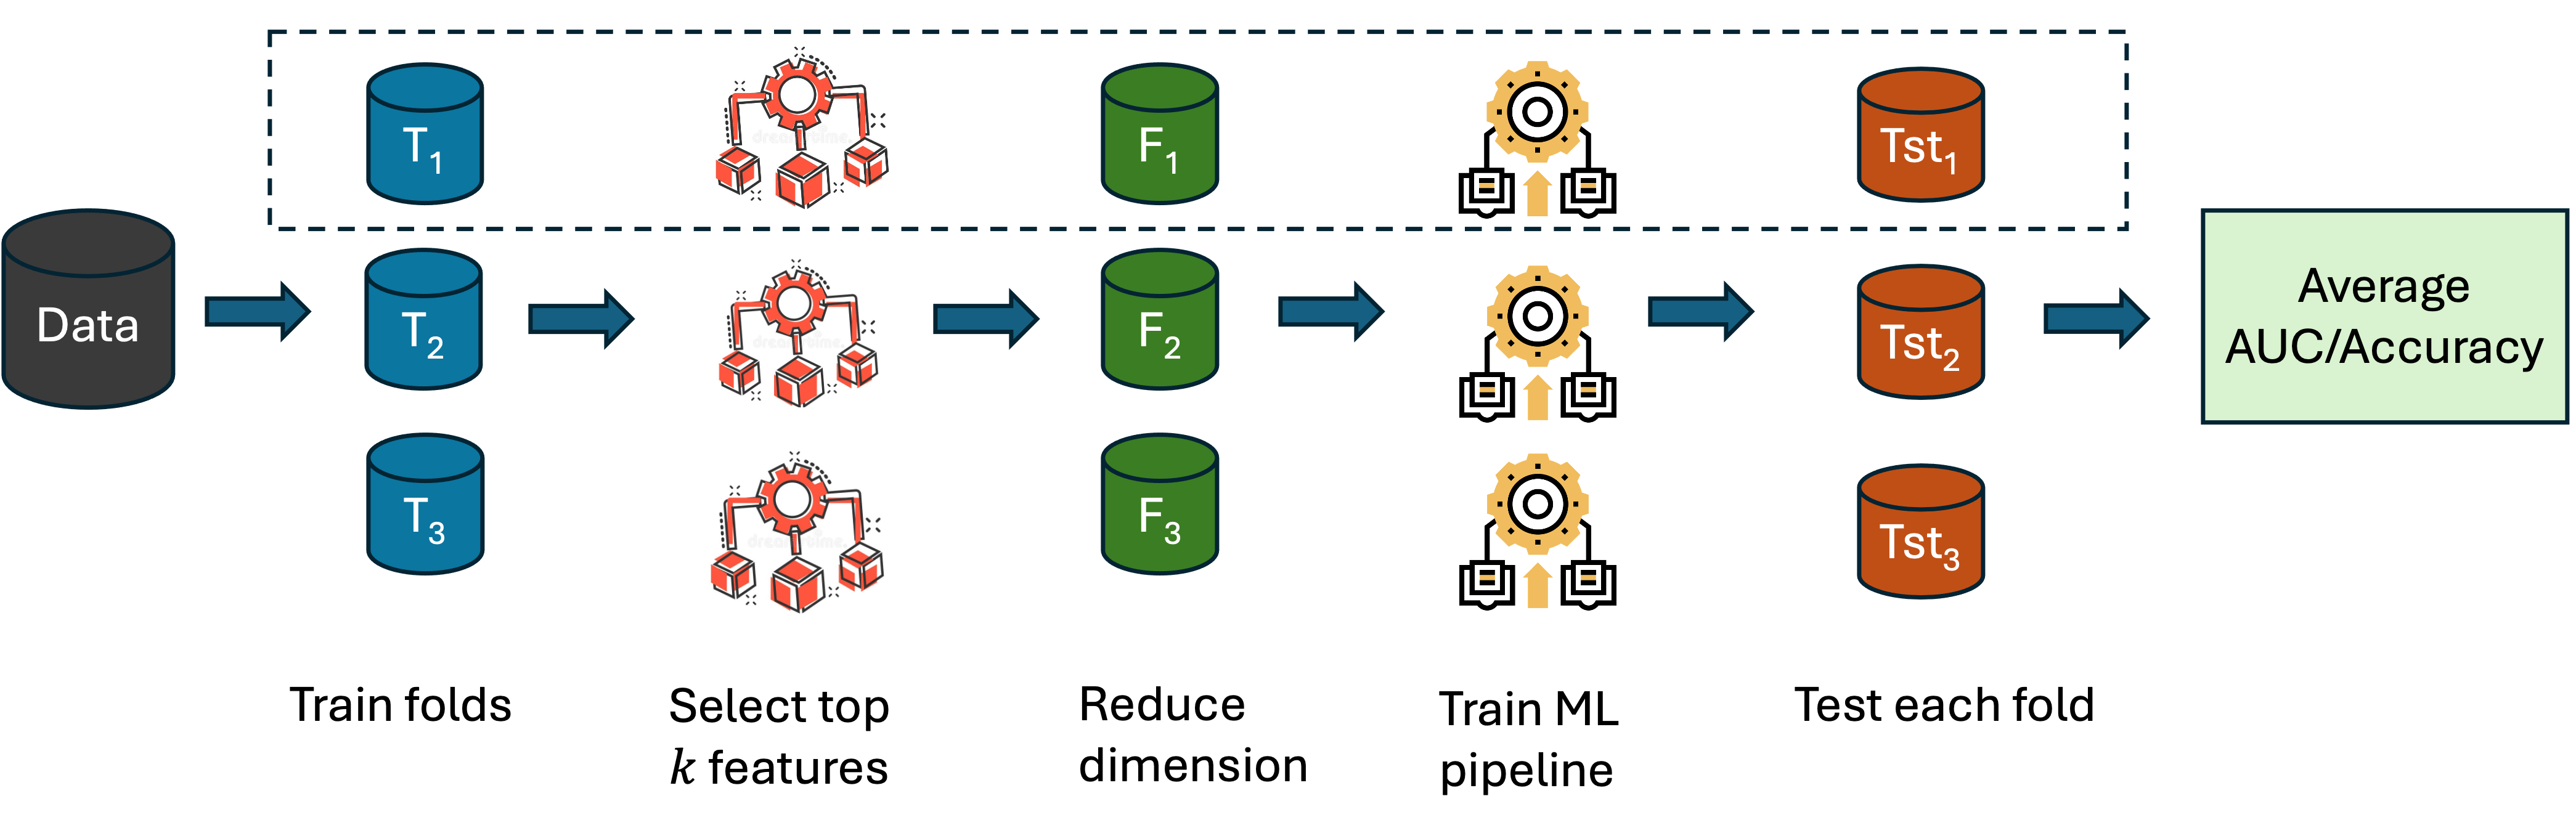
\includegraphics[height=0.32\textwidth]{figures/pipe1.png}
        \caption{The basic pipeline for evaluating a specific FS algorithm on a fixed dataset \(D\) using cross-validation. The figure illustrates 3-CV for brevity, while our experiments used 5-CV. FS is performed separately in each fold \(i\) using \(T_i\), and the reduced fold \(F_i\) is used to train an E-TREE, which is then tested on \(Tst_i\).}
        \label{fig:method_pipeline_a}
    \end{subfigure}
    
    \vspace{1em} % Adjust spacing between subfigures

    % Bottom part (b)
    \begin{subfigure}[t]{0.9\textwidth}
        \centering
        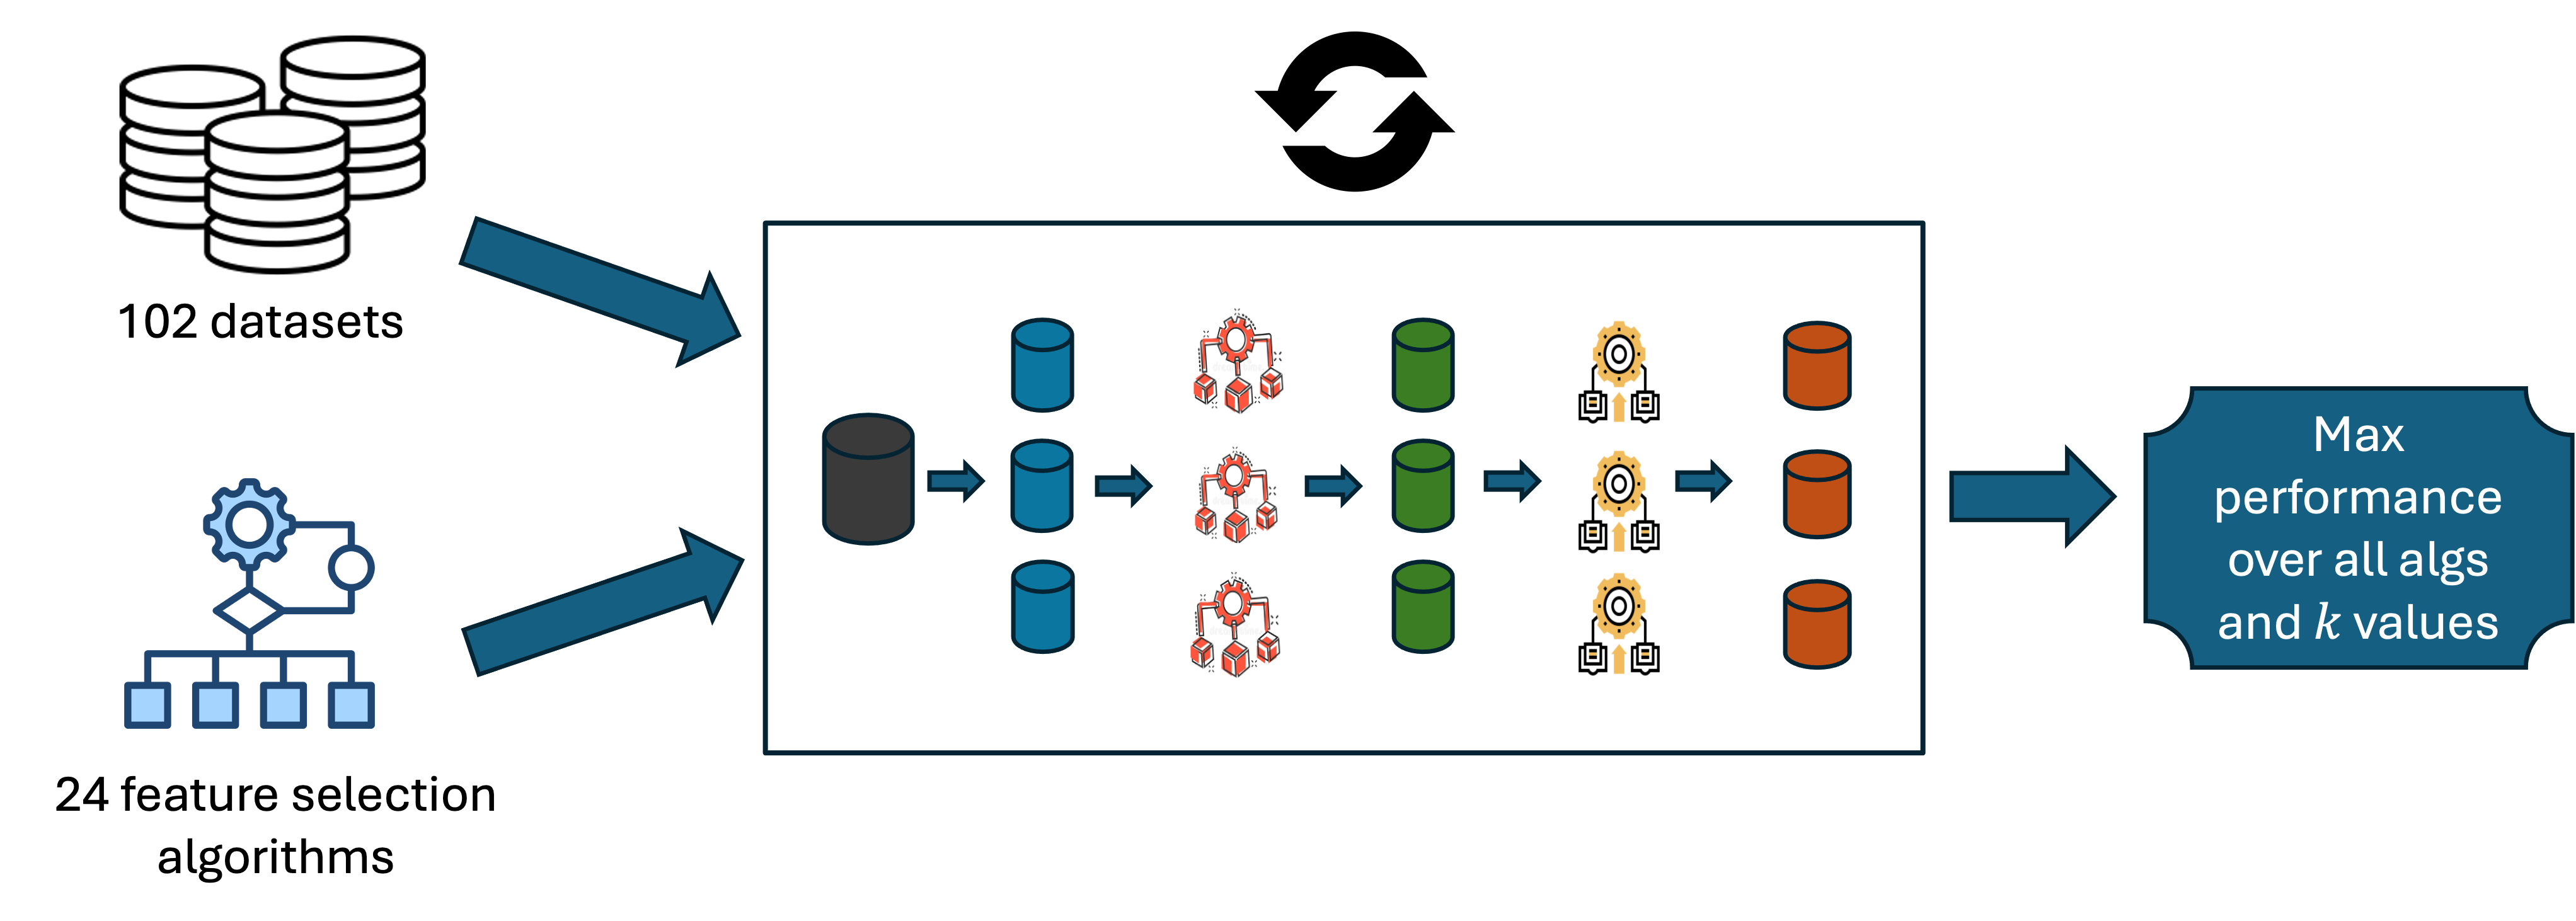
\includegraphics[height=0.35\textwidth]{figures/pipe2.png} % Replace with your bottom image file
        \caption{For a fixed dataset $D$, the pipeline in (a) is repeated for all 27 FS algorithms. The maximum performance is recorded for $D$.}
        \label{fig:method_pipeline_b}
    \end{subfigure}
    
    \caption{The pipeline in (b) is used to categorize a dataset according to Table \ref{tab:dataset_difficulty}. Pipeline (a) is run once without FS ($k=p$) and then repeated all for 27 FS algorithms in Table \ref{tab:FS_algs}, with the number of features $k=1,5,10,30,60$. The best results are used to select the category from Table \ref{tab:dataset_difficulty}.}
    \label{fig:method_pipeline}
\end{figure}


\begin{table}[h!]
\centering \caption{Categorization of a machine learning pipeline performance.Cut-off values were retrieved from leading blogs and papers \cite{Jim_nez_Valverde_2011,lavazza2023reliability}.}
\begin{tabular}{|c|c|c|}
\hline
\textbf{ML Pipeline Performance} & \textbf{AUC Range} \\
\hline
High & AUC $ \geq 90\%$  \\ \hline
Fair & $70\% \le \text {AUC} \le 90\%$ \\ \hline
Low &  AUC$ \leq 70\%$   \\ 
\hline 
\end{tabular}

\label{tab:category_cutoff}
\end{table}

Let us note that Hosmer et al.~\cite{hosmer2013applied} propose a four-tier interpretation of AUC values: \textit{poor} (50\%--70\%), \textit{acceptable} (70\%--80\%), \textit{excellent} (80\%--90\%), and \textit{outstanding} (90\%--100\%). However, other sources, including \cite{corbacioglu2023roc,Jim_nez_Valverde_2011,lavazza2023reliability}, tend to reserve the term \textit{excellent} for performance above 90\%, often merging the 80\%-90\% range with the broader \textit{moderate} or \textit{acceptable} category. To maintain consistency with this more conservative usage and to improve clarity and usability, we opted for a simplified three-category scheme where the 80\%--90\% AUC range is grouped with the medium category.


Now we are ready to combine Q1+Q2 and Table \ref{tab:category_cutoff} to obtain the classification rules for the discrete categories. The categorization rules in Table \ref{tab:dataset_difficulty} reflect the following logic: The top three rules reflect the principle that applying FS results in performance remaining in at least the same category as without FS, aligning with the hierarchy where High, Fair, and Low performance correspond to the Easy, Medium, and Hard categories, respectively. The 'Fragile' category, on the other hand, captures all cases where FS negatively impacts performance.

Having established the empirical categorization rules, we now turn back to the dataset-complexity indicators of \cite{ho2002complexity}, which provides a theoretical foundation for interpreting dataset difficulty in terms of intrinsic data properties. In previous studies, these dataset-complexity indicators were not used to rank datasets by hardness, primarily because no ground truth existed to anchor such a ranking. Instead, these measures were typically employed in an exploratory fashion, providing descriptive insights into the distribution of dataset properties across benchmark collections. Following this rationale, we use the 22 complexity measures implemented in the \href{https://github.com/w4k2/problexity?utm_source=chatgpt.com}{\texttt{problexity}} repository \cite{problexity} to support and validate our empirical categorization. Specifically, we examine how and to what extent the 22 intrinsic data characteristics correspond to the categorical partition induced by Table~\ref{tab:dataset_difficulty}, thereby assessing whether the observed difficulty levels reflect underlying dataset properties rather than artifacts of limited algorithmic coverage or implementation choices. A detailed analysis of these relationships is presented in Section~\ref{sec:intrinsic}.




\begin{table}[h!]
\centering \caption{Categorization of dataset difficulty based on ML pipeline performance, as defined in Table \ref{tab:category_cutoff}. The governing logic for the top three rows is that FS doesn't effect performance adversely; 'Fragile' captures the opposite scenario.}
\begin{tabular}{|c|c|c|}
\hline
\textbf{Dataset Category} & Performance without FS (Q1) & Performance with FS (Q2)  \\ \hline
\textbf{Easy} & Low, Fair, High & High \\ \hline
\textbf{Medium} & Low, Fair & Fair \\ \hline
\textbf{Hard} & Low & Low  \\ \hline  \hline
\textbf{Fragile} & 
\begin{tabular}[c]{@{}c@{}}  High\\ Fair\end{tabular} & 
\begin{tabular}[c]{@{}c@{}}Fair or Low \\ Low \end{tabular} \\ \hline
\end{tabular}

\label{tab:dataset_difficulty}
\end{table}


We conclude this section with an important aspect of our framework. The categorization of a specific dataset is with respect to a given set of ML and FS algorithms that were used to categorize it. Therefore, this categorization is dynamic and invites researchers to challenge and keep updating the assigned categories (note that updates are always upwards, and that 'Easy' cannot be updated by definition). To support this dynamic nature, we run a Power-BI platform where we constantly add more algorithms and datasets and keep track of the most recent categories. The Power-BI tool also allows the change of the cut-offs defined in Table \ref{tab:category_cutoff}, and accordingly, the categories change on the fly. This platform can be approached at \url{HTTP://afteracceptance.com}.



{\footnotesize

\begin{longtable}[H]
{|c|p{1.7cm}|p{7.9cm}|p{1cm}|p{0.8cm}|p{0.8cm}|p{0.8cm}|}
%{|c|l|l|c|c|c|c|}
\caption{Binary datasets, grouped by category. The Category is taken from the paper where the dataset was presented or the repository from where it was downloaded. The Majority column gives the size of the majority class.} \label{tab:Binary Y label Datasets} \\
\hline
{ \textbf{\#}} & { \textbf{Category}} & { \textbf{Dataset}} & { \textbf{Year}} & { \textbf{p}} & {\textbf{n}} & {\textbf{MAJ}} \\
\hline
\endfirsthead

\multicolumn{7}{c}%
{{\bfseries Table \thetable\ continued from previous page}} \\
\hline
{ \textbf{\#}} & {\textbf{Category}} & { \textbf{Dataset}} & { \textbf{Year}} & { \textbf{p} & {\textbf{n}} & { \textbf{MAJ}} \\
\hline
\endhead

\hline \multicolumn{7}{|r|}{{Continued on next page}} \\ \hline
\endfoot

\hline
\multicolumn{7}{| r |}{End of Table}\\
\hline
\endlastfoot


1 & Biological & Heart\_Stalog \cite{statlog_(heart)_145} & 2019 & 13 & 270 & 56\% \\
2 & Biological & Bioresponse \cite{vanschoren2014openml} & 2012 & 1776 & 3751 & 54\% \\
3 & Biological & Period\_Changer \cite{period_changer_729} & 2022 & 1177 & 90 & 70\% \\ \hline 
4 & Gene & Promoters \cite{yilmaz2023mucsteri} & 2023 & 59 & 106 & 50\% \\
5 & Gene & colon \cite{alon1999broad} & 1999 & 2000 & 62 & 65\% \\
6 & Gene & CNS \cite{pomeroy2002prediction} & 2002 & 7129 & 60 & 65\% \\
7 & Gene & leukemia \cite{li2017feature} & 2021 & 7070 & 72 & 65\% \\
8 & Gene & Ovarian \cite{petricoin2002use} & 2014 & 15154 & 253 & 64\% \\
9 & Gene & Breast \cite{pochet2004systematic} & 2004 & 24481 & 97 & 53\% \\
10 & Gene & SMK-CAN-187 \cite{li2017feature} & 2006 & 19993 & 187 & 52\% \\
11 & Gene & ALLAML \cite{golub1999molecular} & 1999 & 7129 & 72 & 65\% \\
12 & Gene & AP\_Prostate\_Lung \cite{stiglic2010stability} & 2010 & 10936 & 195 & 65\% \\
13 & Gene & AP\_Omentum\_Uterus \cite{stiglic2010stability} & 2010 & 10936 & 201 & 62\% \\
14 & Gene & AP\_Breast\_Uterus \cite{stiglic2010stability} & 2010 & 10936 & 468 & 74\% \\
15 & Gene & AP\_Breast\_Kidney \cite{stiglic2010stability} & 2014 & 10936 & 604 & 57\% \\
16 & Gene & AP\_Colon\_Kidney \cite{stiglic2010stability} & 2014 & 10936 & 546 & 52\% \\
17 & Gene & AP\_Ovary\_Uterus \cite{stiglic2010stability} & 2014 & 10936 & 322 & 61\% \\
18 & Gene & AP\_Colon\_Omentum \cite{stiglic2010stability} & 2014 & 10936 & 363 & 79\% \\
19 & Gene & AP\_Uterus\_Kidney \cite{stiglic2010stability} & 2010 & 10936 & 384 & 68\% \\
20 & Gene & AP\_Colon\_Ovary \cite{stiglic2010stability} & 2014 & 10936 & 484 & 59\% \\
21 & Gene & AP\_Omentum\_Kidney \cite{stiglic2010stability} & 2014 & 10936 & 337 & 77\% \\
22 & Gene & AP\_Colon\_Prostate \cite{stiglic2010stability} & 2014 & 10936 & 355 & 81\% \\
23 & Gene & AP\_Omentum\_Ovary \cite{stiglic2010stability} & 2014 & 10936 & 275 & 72\% \\
24 & Gene & AP\_Endometrium\_Breast \cite{stiglic2010stability} & 2014 & 10936 & 405 & 85\% \\
25 & Gene & AP\_Ovary\_Kidney \cite{stiglic2010stability} & 2010 & 10936 & 187 & 67\% \\
26 & Gene & AP\_Endometrium\_Lung \cite{stiglic2010stability} & 2010 & 10936 & 187 & 67\% \\
27 & Gene & AP\_Prostate\_Kidney \cite{stiglic2010stability} & 2014 & 10936 & 329 & 79\% \\
28 & Gene & AP\_Endometrium\_Ovary \cite{stiglic2010stability} & 2010 & 10936 & 259 & 76\% \\
29 & Gene & AP\_Prostate\_Uterus \cite{stiglic2010stability} & 2014 & 10936 & 193 & 64\% \\
30 & Gene & AP\_Breast\_Colon \cite{stiglic2010stability} & 2010 & 10936 & 630 & 55\% \\
31 & Gene & AP\_Breast\_Ovary \cite{stiglic2010stability} & 2010 & 10936 & 542 & 63\% \\
32 & Gene & AP\_Breast\_Lung \cite{stiglic2010stability} & 2010 & 10936 & 470 & 73\% \\
33 & Gene & AP\_Breast\_Prostate \cite{stiglic2010stability} & 2010 & 10936 & 384 & 68\% \\
34 & Gene & AP\_Breast\_Omentum \cite{stiglic2010stability} & 2014 & 10936 & 421 & 82\% \\
35 & Gene & AP\_Lung\_Uterus \cite{stiglic2010stability} & 2014 & 10936 & 250 & 50\% \\
36 & Gene & AP\_Endometrium\_Prostate \cite{stiglic2010stability} & 2014 & 10936 & 130 & 53\% \\
37 & Gene & AP\_Lung\_Kidney \cite{stiglic2010stability} & 2010 & 10936 & 386 & 67\% \\
38 & Gene & AP\_Omentum\_Lung \cite{stiglic2010stability} & 2014 & 10936 & 203 & 62\% \\
39 & Gene & DLBCL \cite{shipp2002diffuse} & 2002 & 5470 & 77 & 75\% \\
40 & Gene & HIVA \cite{guyon2006performance} & 2007 & 1617 & 4229 & 96\% \\
41 & Gene & Prostate-GE \cite{li2017feature} & 2020 & 5966 & 102 & 51\% \\
42 & Gene & GLI-85 \cite{freije2004gene} & 2006 & 22283 & 85 & 69\% \\
43 & Gene & Genbase \cite{diplaris2005protein} & 2005 & 1185 & 662 & 88\% \\
44 & Gene & tumors\_C \cite{pomeroy2002prediction} & 2014 & 7129 & 60 & 65\% \\ \hline 
45 & Healthcare & hepatitis \cite{hepatitis_46} & 1983 & 19 & 154 & 55\% \\
46 & Healthcare & Arrhythmia \cite{arrhythmia_5} & 1997 & 279 & 452 & 54\% \\
47 & Healthcare & Heart\_Disease \cite{zhang2018integrating} & 2021 & 13 & 1025 & 51\% \\ \hline 
48 & Imaging & gisette \cite{guyon2004result} & 2004 & 5000 & 7000 & 50\% \\
49 & Imaging & darwin \cite{cilia2018experimental} & 2022 & 450 & 174 & 51\% \\
50 & Imaging & GINA \cite{guyon2006performance} & 2007 & 970 & 3468 & 51\% \\ \hline 
51 & Text & BASEHOCK \cite{li2017feature} & 2017 & 4862 & 1993 & 50\% \\
52 & Text & slashdot \cite{read2011classifier} & 2020 & 1079 & 3782 & 98\% \\
53 & Text & PCMAC \cite{li2017feature} & 2017 & 3289 & 1943 & 51\% \\
54 & Text & RELATHE \cite{li2017feature} & 2017 & 4322 & 1427 & 55\% \\
55 & Text & spambase \cite{spambase_94} & 1999 & 57 & 4600 & 61\% \\ \hline 
56 & Chemical & biodegradation \cite{mansouri2013quantitative} & 2013 & 41 & 1055 & 66\% \\
57 & Chemical & Musk2 \cite{musk_(version_2)_75} & 1994 & 166 & 6598 & 85\% \\ \hline 
58 & Other & arcene \cite{guyon2004result} & 2004 & 10000 & 200 & 56\% \\
59 & Other & madelon \cite{guyon2004result} & 2004 & 500 & 2600 & 50\% \\
60 & Other & Titanic \cite{ekinci2018comparative} & 2015 & 9 & 891 & 62\% \\
61 & Other & dbworld bodies \cite{dbworld_e-mails_219} & 2011 & 4702 & 64 & 55\% \\
62 & Other & dbworld-bodies-stemmed \cite{filannino2011dbworld} & 2015 & 3721 & 64 & 55\% \\
63 & Other & Ringnorm \cite{breiman1996bias} & 2015 & 20 & 7400 & 50\% \\

%\caption*{\small \textit{64 Binary Y label datasets in our repository, sorted by category and number of citations.}}
\end{longtable}

}

\section{Dataset repository}\label{sec:dataset}
We curated a repository of 102 datasets from different domains. The primary selection criteria were (1) datasets that were used in highly cited feature selection surveys and method papers, (2) searching with keywords such as "high-dimensional datasets," "complex datasets for feature selection," and "dataset with the curse of dimensionality," (3) using open repositories like \href{https://www.kaggle.com/}{Kaggle}, \href{https://archive.ics.uci.edu/ml/index.php}{UCI}, \href{https://www.openml.org/}{OpenML}, \href{https://zenodo.org/}{Zenodo}, \href{https://www.ncbi.nlm.nih.gov/geo/}{NCBI}, and more. (4) dataset for which poor classification performance was reported in the literature.

Table \ref{tab:Binary Y label Datasets} details the 63 binary target-variable datasets. The remaining 39 datasets, described in Table \ref{tab:multiclass_data} in the Appendix,  are non-binary, with class counts ranging from 3 to 50. Figure \ref{fig:data_per_class} shows the number of datasets per class count.  For convenience, we have made the datasets available on our GitHub\footnote{{\url{https://github.com/ItamarEl/FeatureSelect-Benchmark-Hubהפוך תחת שולן
}}.}




%Table \ref{tab:datasets_multiclass_auc} in the Appendix contains more information about all datasets, specifically the repository name from which the dataset was taken.



\begin{figure}[H]
    \centering 
    
\includegraphics[height=0.32\textwidth
    ]{figures/Overview of Dataset by Number of Classes.png}
    \caption{Overview of 102 datasets by number of classes}
    \label{fig:data_per_class}
\end{figure}



% The datasets were sourced from several prominent repositories, known for their rich and diverse data collections. These include: 
% \begin{enumerate}
%     \item \href{https://www.kaggle.com/}{Kaggle},
%     \item \href{https://archive.ics.uci.edu/ml/index.php}{UCI},
%     \item \href{https://www.openml.org/}{OpenML},
%     \item \href{https://web.archive.org/web/20130512034606/http:/www.nipsfsc.ecs.soton.ac.uk/datasets/}{NIPS 2003},
%     \item \href{https://zenodo.org/}{Zenodo},
%     \item \href{https://jundongl.github.io/scikit-feature/}{scikit-feature},
%     \item \href{https://www.agnostic.inf.ethz.ch/datasets.php}{WCCI 2006},
%     \item \href{http://www.gems-system.org/}{GEMS},
%     \item \href{https://www.ncbi.nlm.nih.gov/}{NIH}, and
%     \item \href{https://www.ncbi.nlm.nih.gov/geo/}{NCBI}.
% \end{enumerate}

% Originally, these datasets were found in various file formats such as ARFF, Excel, CSV, and MAT, reflecting the wide-ranging practices of data sharing and documentation in different research communities. To standardize our dataset repository for consistent access and analysis, all datasets were converted into a uniform MATLAB (.mat) format. In this format, feature sets are stored in \( X \) and label vectors in \( Y \), facilitating straightforward integration into analytical workflows and machine learning model training processes.


\section{Experimental Setting}\label{sec:exp_setting}

We now provide the missing details of the methodology, completing the description of both the machine learning pipeline and the FS algorithms used. This expands on the process outlined in Figure~\ref{fig:method_pipeline} and formalizes the categorization procedure according to the rules defined in Table~\ref{tab:dataset_difficulty}.

\subsection{ML Pipeline} \label{sec:ml_flow}
In this study, we focus on labeled tabular data, for which the standard modeling choice is typically a decision-tree-based ensemble algorithm~\cite{grinsztajn2022tree}. We adopt \emph{Extremely Randomized Trees} (E-Tree)~\cite{geurts2006extremely}, a widely recognized baseline due to its strong predictive performance, computational efficiency—especially valuable in high-dimensional settings—and reduced variance from randomized splits~\cite{geurts2006extremely}. Its robustness has been demonstrated across various domains, including bioinformatics~\citep{kocev2020ensembles}, clinical risk prediction~\citep{sutradhar2023boo}, and FS benchmarking~\citep{atashgahi2022quick}. In preliminary comparisons with Random Forest and AdaBoost~\cite{freund1997decision}, E-Tree performed comparably or better, further supporting its use as our default choice.

We ran three variants of  \href{https://scikit-learn.org/dev/modules/generated/sklearn.ensemble.ExtraTreesClassifier.html}{E-Tree} that differ in \texttt{max\_depth}, the maximum tree depth, and \texttt{n\_estimators}, the number of trees. The parameter pairs we tested were (3,100), (3,200), and (5,100). The remaining parameters were left at their default value.



Our evaluation strategy follows a two-stage screening process. In the first stage, we apply the E-Tree pipeline across all datasets to obtain initial dataset category. If a dataset is labeled as 'Easy', no further testing is needed. However, if a dataset is initially labeled as 'Medium' or 'Hard', this may reflect a misalignment between E-Tree and the dataset’s underlying structure rather than genuine difficulty. To control for this possibility, we enter a second stage: rerunning the evaluation pipeline using a diverse set of classifiers that represent distinct algorithmic principles—generalized linear models (Logistic Regression), margin-based methods (SVM), non-parametric approaches (KNN), and alternative ensemble learners (Random Forest, XGBoost). The category is set by the best result obtained in the multi-classifier pipeline. 

\subsection{Execution Flow}\label{sec:execution_flow}

Recall that to apply the rules of Table \ref{tab:dataset_difficulty} we need to compute the performance metrics with and without FS (Q1 and Q2 in Section \ref{sec:methodology}).

%As detailed in table \ref{tab:Detailed Information of Feature Selection Algorithms Reviewed in the Article}, we utilized a combination of sources for our feature selection algorithms. Some algorithms were taken directly from the default implementations provided in well-known Python libraries such as scikit-learn and SciPy. Others, specifically CT, DT, and LeadingEV, were custom-implemented by our team where we wrote the logic and coded the algorithms ourselves.


The execution flow, illustrated in Figure 
\ref{fig:method_pipeline}, was identical for all datasets $D$, FS algorithms $A$, and the number of features $k \in \{1,5,10,30,60,p\}$ (when $k=p$ then no FS is performed). So let us fix $D,A,k$, and do the following:
\begin{enumerate}
    \item Split $D$ into five train-test folds, $D_1-D_5$.
    \item For each fold $D_i$, run $A$  on the fold's train to obtain the $A$'s selected feature set $F_i$ of size $k$.
    \item Reduce $D_i$ to the features $F_i$ and train the ML pipeline .
    \item Test the ML pipeline on the fold's test. 
    \item Record the average performance metrics over the three folds for each ML classifier and take the best one.
\end{enumerate}

When steps 1--5 were executed for all 27 FS algorithms, we took the maximum performance metric over all 27 algorithms (Q2) and compared it with the $k=p$ execution (Q1). 
We used Table \ref{tab:category_cutoff} to get the discrete performance category and then derive the dataset hardness category according to Table \ref{tab:dataset_difficulty}.

Steps 1--5 were executed twice. One time, just with E-Tree; all 'Easy' datasets were removed from the pool, and then steps 1--5 were repeated for the remaining datasets with the multi-classifier pipeline.

\vspace{3.5}

% \begin{itemize}
%     \item The use of the `max` function in this scheme, both across E-Tree variants and the 24 FS algorithms, is crucial for ensuring a robust and fair evaluation of dataset hardness. By taking the maximum performance across the E-Tree variants, we account for the best possible outcome within the given modeling framework, avoiding penalization due to the sub-optimal parameter choice of any specific E-Tree model. Similarly, by taking the maximum across the 24 FS algorithms, we identify the highest achievable performance on the dataset using any feature selection method. This ensures that the evaluation focuses on the dataset's intrinsic difficulty rather than the performance variability of specific algorithms or models. If, even under these most favorable conditions, the dataset's performance remains poor, it  supports its classification as "Hard." 

The choice of $k \in \{1, 5, 10, 30, 60 \}$ in our study reflects a pragmatic balance between empirical insights from the literature, practical considerations, and the diversity of feature selection (FS) applications. Studies such as \cite{bertolini2021enhancing} for educational data mining has shown that optimal feature subset of size 7-9 features out of 32. In domains like protein structure prediction, \cite{Yi_2022}  have adopted more granular evaluations with \(k\) values like 10, 20, 30, 40, and 50. The default value of scikit-learn's popular SelectKBest is $k=10$. Our choice of \(k\) incorporates both small subsets (1, 5, 10) to test the algorithms' ability to select highly informative features while also including larger subsets (30, 60) to evaluate performance when more features are retained. 



We note that a few FS algorithms in our study, specifically Alpha Investing, SHAP, CEI\_GA, and SVC, employ internal stopping criteria and may return fewer than $k$ features. In such cases, we used the exact subset returned by the algorithm, without padding it to reach $k$. For example, if an algorithm returned 34 features, then when $k=1,5,30$ we took the first $k$ features and when $k=60$ we evaluated the set of 34 features as-is. Importantly, we did not encounter any case where an algorithm returned more than 60 features.

\subsection{FS Algorithm Parametrization}
One of the key factors that influences the performance of feature selection algorithms is the selection of hyperparameters. Typically, the data is partitioned into train and test sets, where the train set is further partitioned into smaller subsets to allow for hyperparameter tuning through grid search or similar techniques. However, in our case, this approach is not feasible due to the sheer volume of datasets and algorithms being evaluated, as well as the small size of some datasets, which makes further partitioning impractical. 

To circumvent this obstacle, we first opted to use the parameters recommended in the respective resources for algorithms sourced from repositories like GitHub or Python packages such as scikit-learn. To ensure the reliability of these choices, we conducted a preliminary grid search on five randomly selected datasets to verify that the reported parameters yielded comparable performance in our setup. The full list of parameters per algorithm can be found in our GitHub repository alongside the code.

In cases where the source did not explicitly specify parameter values, we selected the best-performing configuration from the grid search. For in-house algorithms, the only method requiring parameter tuning was Covariance Thresholding (CT), which has a single parameter, the threshold (\(T\)). We set this threshold to \(T=1\). 

Notably, the majority of datasets in our study were categorized as 'Easy'. This finding highlights that exploring additional parameter configurations for the FS algorithms or E-Tree models would not have significantly altered our key results. Such additional parameter tuning can only bump the category of a dataset, say from 'Medium' to 'Easy', and certainly not introduce new 'Hard' datasets. 
Therefore, our key finding remains robust and withstands the claim for limited hyperparameter tuning.



\subsection{Performance Metrics}

We chose AUC as our primary performance metric due to its robustness across class distributions and decision thresholds. A recent systematic \cite{li2024area} compared 18 evaluation metrics across 156 binary classification scenarios and found that AUC consistently exhibited the lowest variance in both individual model evaluation and model ranking. Because AUC considers all possible decision thresholds, it is less sensitive to prevalence and better suited for generalized comparisons. 


In addition to AUC, we report accuracy on a subset of 33 nearly balanced binary datasets, where the majority class comprises 50\%-60\% of the samples. For these datasets, accuracy is more interpretable, and we include a discussion of the few discrepancies in dataset categorization observed when comparing AUC and accuracy-based results. However, we note that the overall findings remain consistent, underscoring the robustness of our conclusions.

As for alternative metrics, we argue that AUC and accuracy (for nearly balanced datasets) are sufficient for our analysis. While F1-score is often used as a perofrmance metric, it is disproportionately influenced by the majority class unless specifically calculated for the minority class. However, this level of granularity, while informative, introduces additional specificity that goes beyond the scope of our current study. Thus, while we acknowledge the potential value of such metrics in other contexts, AUC remains the most appropriate and generalizable choice for our work.

When evaluating performance for multi-class datasets, we use the One-vs-Many (OVM) AUC. The OVM AUC extends the concept of binary AUC to multi-class settings by computing an AUC score for each class by treating it as the "positive" class and all other classes as the "negative" class. The final OVM AUC is the average across all classes.




\subsection{Hardware and Running Time}
All experiments were conducted on a GPU-cluster equipped with:
\begin{itemize}
    \item 10x RTX A5000 GPUs
    \item 512 GB RAM
    \item 2x AMD EPYC 7443 24-Core Processors
\end{itemize}

We conducted approximately 11,000 experiments involving 5-fold cross-validation on 102 datasets. These experiments were run in parallel across the different $k$ values (1, 5, 10, 30, 60, $p$) across the 27 algorithms. The running times varied significantly, with some algorithms completing in less than 30 seconds and others requiring several days on our computing cluster. 



\section{Results}\label{sec:results}
Table \ref{tab:binary_dataset_complexity} gives the outcomes of the execution flow described in Section \ref{sec:exp_setting}. The findings are quite straightforward: we found no 'Hard' datasets, 11 'Medium', and 52 'Easy'. Out of the 'Easy', four (colored in green) were classified as 'Easy' only in the second stage when applying the multi-classifier pipeline.

One can also observe that the performance of the majority of the 'Medium' datasets is far from the 'Easy' cutoff (90\%), supporting the choice of cut-offs.

Out of the 39 multiclass datasets, three were 'Medium' and 36 'Easy' - same trend as in the binary datasets (Table \ref{tab:datasets_multiclass_auc}).

When repeating the evaluation with accuracy instead of AUC, for nearly-balanced binary datasets, we got very similar results. Among the 33 nearly-balanced binary datasets, there were only three discrepancies with AUC (three 'Medium' by accuracy but 'Easy' by AUC: Arcene, Arrhythmia, and Heart\_Stalog). Details in Table \ref{tab:complete_dataset_analysis_acc}

We found no 'Fragile' datasets, binary or multi-class, using AUC or accuracy.


Finally, Table \ref{tab:non_balanced_dataset_analysis_acc} summarizes the accuracy performance for the non-balanced multi-class and binary datasets, but without categorization. Future work that will define more nuanced complexity categorization can make use of our raw data to extract meaningful categorization. 

\vspace{2mm}
While we found no 'Hard' datasets, such benchmarks are valuable for developers of FS algorithms to justify new methods and for authors of FS reviews and surveys to select benchmarks in an informed and impactful manner. To address this gap, two potential approaches can be pursued: the first is to generate synthetic hard datasets, as explored in the literature for creating controlled evaluation scenarios, and the second is to identify subsets of real-world datasets that form 'Hard' datasets. The procedure for this second approach is detailed in the next section.




\definecolor{HardCol}{RGB}{180,0,0}     % darker red
\definecolor{MedCol} {RGB}{200,100,0}   % darker orange
\definecolor{EasyCol}{RGB}{0,120,0}     % darker green


{\footnotesize
\begin{longtable}{|>{\raggedright\arraybackslash}p{0.3cm}|>{\raggedright\arraybackslash}l|>{\raggedright\arraybackslash}p{3.5cm}|>{\raggedright\arraybackslash}p{3.5cm}|>{\raggedright\arraybackslash}c|}
\caption{Binary dataset complexity categorization. Datasets are grouped by category and sorted within each category by FS AUC performance.} \label{tab:binary_dataset_complexity} \\
\hline
\textbf{\#} & \textbf{Dataset} & \textbf{AUC (Performance)} & \textbf{FS AUC (Perform.)} & \textbf{Category} \\
\hline
\endfirsthead

\multicolumn{5}{c}%
{{\bfseries \tablename\ \thetable{} -- continued from previous page}} \\
\hline
\textbf{\#} & \textbf{Dataset} & \textbf{AUC (Performance)} & \textbf{FS AUC (Perform.)} & \textbf{Category} \\
\hline
\endhead

\hline \multicolumn{5}{r}{{Continued on next page}} \\ \hline
\endfoot

\hline
\endlastfoot
\noalign{\vskip 1pt}
1 & Period Changer & 51.9\% ± 16.90\% (Low) & 71.2\% ± 12.4\% (Fair) & Medium \\
2 & slashdot & 75.2\% ± 4.90\% (Fair) & 73.0\% ± 5.1\% (Fair) & Medium  \\
3 & tumors\_C & 62.4\% ± 18.00\% (Low) & 74.3\% ± 18.1\% (Fair) & Medium \\
4 & Breast & 72.6\% ± 12.60\% (Fair) & 75.1\% ± 5.7\% (Fair) & Medium \\ 
5 & hepatitis & 73.4\% ± 6.10\% (Fair) & 75.2\% ± 7.6\% (Fair) & Medium \\
6 & CNS & 62.4\% ± 18.00\% (Low) & 75.8\% ± 18.1\% (Fair) & Medium \\
7 & colon & 56.4\% ± 8.90\% (Low) & 76.4\% ± 14.8\% (Fair) & Medium \\
8 & HIVA & 79.0\% ± 3.10\% (Fair) & 77.4\% ± 7.2\% (Fair) & Medium \\
9 & SMK-CAN-187 & 80.5\% ± 8.00\% (Fair) & 77.8\% ± 10.7\% (Fair) & Medium \\
10 & Bioresponse & 87.3\% ± 2.20\% (Fair) & 86.9\% ± 2.1\% (Fair) & Medium \\
11 & Titanic & 86.5\% ± 2.40\% (Fair) & 84.9\% ± 2.4\% (Fair) & Medium \\ \hline 
12 & AP\_Omentum\_Ovary & 86.8\% ± 4.30\% (Fair) & 91.1\% ± 3.9\% (Fair) &  \color{EasyCol} Easy \\ 
\noalign{\vskip 1pt}
13 & arcene & 93.7\% ± 3.80\% (Fair) & 90.3\% ± 7.2\% (Fair) & \color{EasyCol} Easy  \\
14 & madelon & 88.2\% ± 2.50\% (Fair) & 94\% ± 2.8\%  (High) & \color{EasyCol} Easy \\ 
15 & Arrhythmia & 88.9\% ± 3.70\% (Fair) & 90.1\% ± 3.2\% (High) & \color{EasyCol} Easy  \\
16 & Musk2 & 90.1\% ± 2.50\% (High) & 91.6\% ± 1.3\% (High) & Easy \\
17 & RELATHE & 91.8\% ± 1.20\% (High) & 90.3\% ± 0.9\% (High) & Easy \\
18 & biodegradation & 90.5\% ± 1.70\% (High) & 90.3\% ± 2.1\% (High) & Easy \\ 
19 & leukemia & 90.1\% ± 8.30\% (High) & 90.3\% ± 4.4\% (High) & Easy \\
20 & Heart\_Stalog & 91.05\% ± 3.50\% (High) & 90.4\% ± 2.8\% (High) & Easy \\
21 & GINA & 92.2\% ± 1.40\% (High) & 91.1\% ± 1.0\% (High) & Easy \\
22 & spambase & 91.0\% ± 1.10\% (High) & 91.9\% ± 0.9\% (High) & Easy \\
23 & dbworld\_bodies & 94.5\% ± 4.80\% (High) & 93.4\% ± 5.4\% (High) & Easy \\
24 & Heart\_Disease & 93.0\% ± 1.60\% (High) & 93.6\% ± 0.8\% (High) & Easy \\
25 & darwin & 94.7\% ± 3.20\% (High) & 93.8\% ± 3.8\% (High) & Easy \\
26 & dbworld-bodies-stemmed & 93.9\% ± 5.20\% (High) & 94.0\% ± 3.4\% (High) & Easy \\
27 & AP\_Endometrium\_Ovary & 94.5\% ± 2.00\% (High) & 94.6\% ± 2.8\% (High) & Easy \\
28 & Ringnorm & 98.8\% ± 0.20\% (High) & 95.0\% ± 0.8\% (High) & Easy \\
29 & PCMAC & 95.3\% ± 1.60\% (High) & 95.2\% ± 1.2\% (High) & Easy \\
30 & AP\_Ovary\_Uterus & 94.6\% ± 1.50\% (High) & 95.4\% ± 1.6\% (High) & Easy \\
31 & AP\_Omentum\_Uterus & 96.3\% ± 2.10\% (High) & 96.3\% ± 1.7\% (High) & Easy \\
32 & GLI-85 & 95.8\% ± 0.80\% (High) & 96.7\% ± 2.8\% (High) & Easy \\
33 & gisette & 96.8\% ± 0.50\% (High) & 96.7\% ± 0.5\% (High) & Easy \\
34 & Prostate-GE & 92.1\% ± 8.40\% (High) & 96.9\% ± 5.3\% (High) & Easy \\
35 & AP\_Colon\_Omentum & 97.6\% ± 1.80\% (High) & 97.0\% ± 2.3\% (High) & Easy \\
36 & ALLAML & 90.4\% ± 9.10\% (High) & 97.6\% ± 3.2\% (High) & Easy \\
37 & AP\_Colon\_Ovary & 97.1\% ± 1.20\% (High) & 97.6\% ± 1.0\% (High) & Easy \\
38 & Promoters & 97.5\% ± 1.80\% (High) & 97.7\% ± 2.6\% (High) & Easy \\
39 & AP\_Breast\_Omentum & 97.4\% ± 2.50\% (High) & 97.9\% ± 1.5\% (High) & Easy \\
40 & DLBCL & 97.9\% ± 3.20\% (High) & 98.3\% ± 3.3\% (High) & Easy \\
41 & AP\_Omentum\_Lung & 98.1\% ± 0.70\% (High) & 98.4\% ± 1.0\% (High) & Easy \\
42 & AP\_Lung\_Uterus & 97.8\% ± 2.20\% (High) & 98.5\% ± 2.3\% (High) & Easy \\
43 & AP\_Breast\_Uterus & 98.6\% ± 0.80\% (High) & 98.6\% ± 0.7\% (High) & Easy \\
44 & BASEHOCK & 99.2\% ± 0.30\% (High) & 98.6\% ± 0.4\% (High) & Easy \\
45 & AP\_Breast\_Lung & 98.0\% ± 1.80\% (High) & 98.7\% ± 1.3\% (High) & Easy \\
46 & AP\_Endometrium\_Breast & 98.9\% ± 1.50\% (High) & 98.8\% ± 0.7\% (High) & Easy \\
47 & AP\_Breast\_Colon & 98.7\% ± 0.90\% (High) & 98.9\% ± 0.7\% (High) & Easy \\
48 & AP\_Endometrium\_Lung & 98.9\% ± 1.00\% (High) & 98.9\% ± 0.8\% (High) & Easy \\
49 & AP\_Ovary\_Kidney & 98.9\% ± 1.00\% (High) & 98.9\% ± 0.8\% (High) & Easy \\
50 & AP\_Breast\_Kidney & 99.2\% ± 0.90\% (High) & 99.3\% ± 0.6\% (High) & Easy \\
51 & AP\_Breast\_Ovary & 99.6\% ± 0.10\% (High) & 99.6\% ± 0.2\% (High) & Easy \\
52 & AP\_Breast\_Prostate & 99.7\% ± 0.10\% (High) & 99.7\% ± 0.2\% (High) & Easy \\
53 & AP\_Lung\_Kidney & 99.7\% ± 0.20\% (High) & 99.7\% ± 0.2\% (High) & Easy \\
54 & AP\_Omentum\_Kidney & 99.7\% ± 0.20\% (High) & 99.7\% ± 0.2\% (High) & Easy \\
55 & AP\_Uterus\_Kidney & 99.7\% ± 0.10\% (High) & 99.7\% ± 0.2\% (High) & Easy \\
56 & AP\_Colon\_Kidney & 99.8\% ± 0.10\% (High) & 99.8\% ± 0.1\% (High) & Easy \\
57 & AP\_Colon\_Prostate & 99.8\% ± 0.20\% (High) & 99.9\% ± 0.2\% (High) & Easy \\
58 & AP\_Prostate\_Kidney & 99.9\% ± 0.10\% (High) & 99.9\% ± 0.2\% (High) & Easy \\
59 & AP\_Prostate\_Lung & 99.5\% ± 0.90\% (High) & 100\% ± 0.0\% (High) & Easy \\
60 & Ovarian & 99.7\% ± 0.60\% (High) & 100\% ± 0.1\% (High) & Easy \\
61 & AP\_Prostate\_Uterus & 99.9\% ± 0.10\% (High) & 100\% ± 0.0\% (High) & Easy \\
62 & Genbase & 100.0\% ± 0.00\% (High) & 100\% ± 0.0\% (High) & Easy \\
63 & AP\_Endometrium\_Prostate & 100.0\% ± 0.00\% (High) & 100\% ± 0.0\% (High) & Easy \\
\end{longtable}
}



% \begin{figure}[H]
%     \centering
%     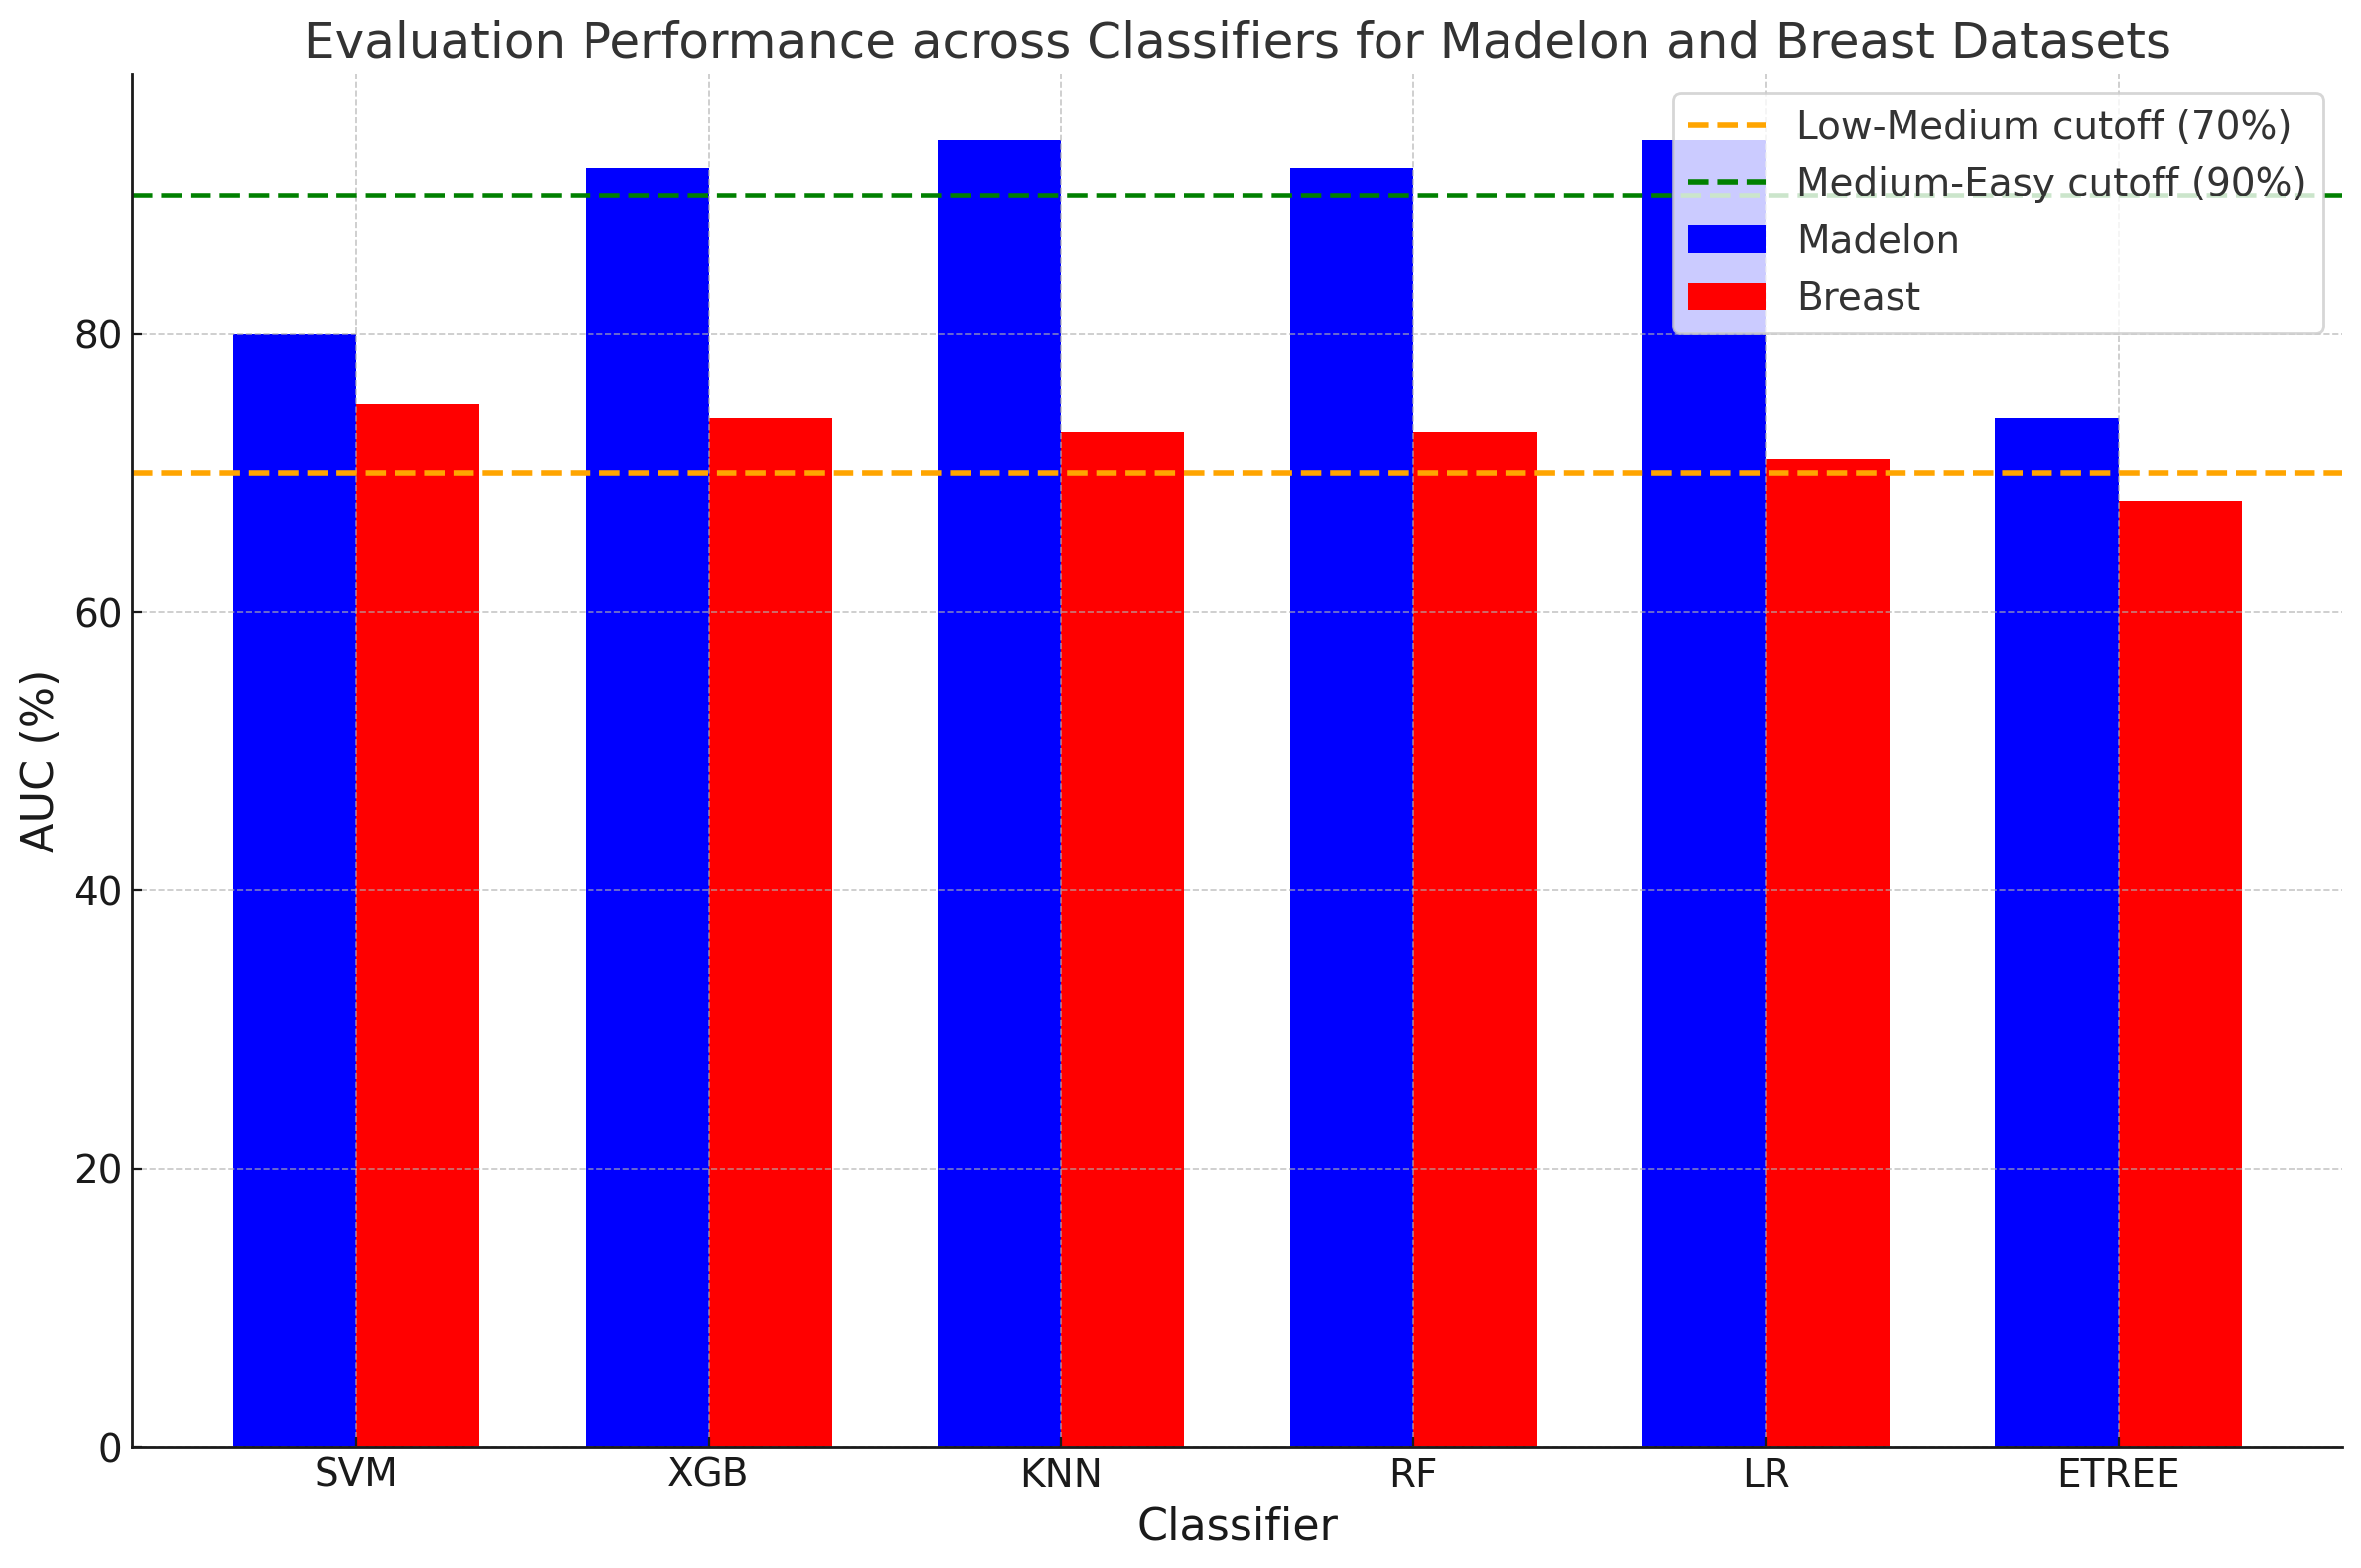
\includegraphics[height=0.45\textwidth]{figures/output (21).png}
%     \caption{Evaluation or performance for the Breast and Madelon datasets across six classifiers. For Madelon, E-Tree was sub-optimal, for Breast a the performance is similar across classifiers. In both cases, the category changes when applying the multiclassifier pipeline, but Breast remains a challenging dataset.}
%     \label{fig:breast_eval}
% \end{figure}




% \begin{table}[h!]
% \centering
% \caption{Ranking of Feature Selection methods by dataset complexity. The count beside each algorithm is the number of datasets where its performance was either the best performance or at most 1 standard deviation away from it.}
% \label{tab:Combined_Ranking_FS}
% \small % smaller font size to fit the table on one page
% \setlength{\tabcolsep}{3pt} % reduce padding between columns
% \begin{tabular}{|c|>{\raggedright\arraybackslash}p{4.5cm}|>{\raggedright\arraybackslash}p{4.5cm}!{\vrule width 1pt}>{\raggedright\arraybackslash}p{4.5cm}|>{\raggedright\arraybackslash}p{4.5cm}|}
% \hline
% \multirow{2}{*}{\textbf{Rank}} & \multicolumn{2}{c!{\vrule width 1pt}}{\textbf{Binary Dataset}} & \multicolumn{2}{c|}{\textbf{All Dataset}} \\ \cline{2-5}
%                                 & \textbf{Easy (49)} & \textbf{Medium (15)} & \textbf{Easy (82)}       & \textbf{Medium (18)}       \\ \hline
% 1                               & ETree (49)         & UnivariateFS (10)    & ETree (80)          & ETree (13)            \\ \hline
% 2                               & mRMR (46)          & AdaBoost (9)         & mRMR (80)           & UnivariateFS (13)     \\ \hline
% 3                               & UnivariateFS (41)  & mRMR (8)             & releifF (75)        & AdaBoost (12)         \\ \hline
% 4                               & AdaBoost (43)      & ETree (8)            & SVC (74)            & mRMR (12)             \\ \hline
% 5                               & releifF (43)       & releifF (7)          & AdaBoost (75)       & releifF (10)          \\ \hline
% 6                               & SVC (39)           & RFS (6)              & UnivariateFS (72)   & RFS (8)               \\ \hline
% 7                               & SVM Forward (39)   & DT (6)               & SVM Forward (69)    & DT (8)                \\ \hline
% 8                               & Alpha Investing (38) & SVC (5)            & DecisionTree (67)   & SVC (8)               \\ \hline
% 9                               & DecisionTree (35)  & Alpha Investing (5)  & CT (64)             & Alpha Investing (7)   \\ \hline
% 10                              & RFS (35)           & DLFS (5)             & RFS (64)            & DLFS (6)              \\ \hline
% \end{tabular}
% \end{table}



\section{Generating Hard Dataset}\label{sec:peeling}
We now describe our procedure for generating real-world 'Hard' datasets.
The input to the hard dataset generator is one of the datasets $D$ in our repository and the output is a tuple $(D_{train},D_{test},F)$, where $D_{train},D_{test}$ are a subset of $D$, and $F$ is a subset of the features of $D$. If the generator returns a tuple $(D_{train},D_{test},F)$ (rather than 'Fail'), the guarantee that we provide on the tuple is:
\begin{enumerate}
    \item  The performance of the multi-classifier pipeline when training on $D_{train}$ and testing on $D_{test}$ is 'Low' (see Table \ref{tab:category_cutoff} to recall 'Low' cutoffs).
    \item All 27 FS algorithms in our repository failed to recover $F$; Furthermore, all feature sets $F'$ that they recovered resulted in 'Low' performance on $D_{test}$.
    \item The size of $D_{\text{train}}$ and $D_{\text{test}}$ is at least 50 and their class balance is as in $D$.
    \item When reducing the features of $D_{train}$ and $D_{test}$ to $F$, then the multi-classifier pipeline, trained on $D_{train}$, obtains 'High' or 'Fair' performance on $D_{test}$.

\end{enumerate}


Guaranteeing the first two properties is rather straightforward, as one can iteratively reduce the size of $D_{train}$ until it's hard to learn the relation between the covariates and the target variable. However, guaranteeing properties 3+4, together with 1+2, is far from trivial. It could very well be that by reducing the size of $D_{train}$ to accommodate properties 1+2, it either became too small or that the ground truth $F$ becomes irrelevant, namely, these features are no longer meaningful. In both cases, $D_{train}$ may be hard, but in a pathological sense, that is not interesting for benchmarking.   

Finally, given a tuple $(D_{train},D_{test},F)$, the challenge for FS algorithm developers is now straightforward: show that your new FS algorithm can recover $F$ from $D_{train}$, or some feature set $F'$ with similar performance to $F$ on $D_{test}$. 

Before detailing the peeling procedure, we note that selectively removing data may risk distorting the dataset’s structure. To mitigate this, we require that the feature subset \(F\), selected prior to peeling, achieves 'High' or 'Fair' performance on the \emph{original} dataset \(D\). This ensures that \(F\) captures genuine signal and that the resulting difficulty stems from the challenge of recovering \(F\), not from data degradation. Furthermore, to preserve representativeness, we enforce a lower bound on dataset size. In the two hard datasets that we produced, see Table \ref{tab:hard_peeled_dataset_summary}, the peeled version retained over 80\% of the original sample size (150/187 and 3026/3782).



\vspace{2mm}


The generation process of candidate $(D_{train},D_{test},F)$ tuples consists of four sub-procedures.
\begin{itemize}
    \item {\bf Split} the dataset $D$ into $D_{train}$ and $D_{test}$, with $D_{train}$ comprising   30\% of the data. Verify that $D_{test}$ is 'Easy' or 'Fair' when the ML pipeline is trained on $D_{train}$, or else return 'Fail'.


\item {\bf Ground Truth Recovery:} Run the 27 FS algorithms on $D_{train}$, with $k=1,5,30,60$, and record the set $\mathcal{F}_{best}$ of feature sets (a set of sets) that scored a 'Fair' or 'High' AUC on $D_{test}$ when evaluated using the multi-classifier pipeline in Section \ref{sec:ml_flow}.

     
    \item {\bf Peeling:} Run an iterative peeling procedure on $D_{train}$ (described below) until the performance of the ML pipeline on $D_{test}$ without FS drops to 'Low'; call $D^*$ this reduced dataset. If the size of $D^*$ is smaller than 50, return 'Fail'.
    \item {\bf Validation:} Check if when training the multi-classifier pipeline on $D^*$, the performance on $D_{test}$ can be restored to 'High' or 'Fair' using (a) FS on $D^*$ or (b) plugging one of the sets $F$ in $\mathcal{F}_{best}$. If the answer to (a) is 'No' and to (b) is 'Yes', output the tuple $(D_{train}:=D^*, D_{test},F)$; otherwise return 'Fail'.
\end{itemize}

 
We now turn to describe the peeling procedure:

{\small
\begin{mdframed}
\textbf{Algorithm: Peeling Procedure}
\begin{algorithmic}[1]
\REQUIRE Training set $D_{\text{train}}$, test set $D_{\text{test}}$, size threshold $\tau$, and performance condition "Low".
\ENSURE The modified $D_{\text{train}}$ after peeling.
\STATE  $\text{status} \gets \text{"Fail"}$.

\While {$|D_{\text{train}}| > \tau$}
    \STATE \hspace{5mm} $D_{\text{train}} \leftarrow$ $D_{\text{train}}$ after randomly removing 10\% from each class.
    \STATE \hspace{5mm} Train multi-classifier pipeline on the trimmed $D_{\text{train}}$.
    \STATE \hspace{5mm} Check the performance of the classifiers on $D_{\text{test}}$.
    \STATE \hspace{5mm} \textbf{if}  {performance is `Low':}
        \STATE \hspace{10mm} $\text{status} \gets \text{"Success"}$.
        \STATE \hspace{10mm} \textbf{break} (stop the peeling process)
    \STATE \hspace{5mm} \textbf{end if}

%\EndWhile
    \STATE \textbf{end while}  % Manually denote the end of the while loop
    \STATE \textbf{return} status % Manually denote the end of the while loop

\end{algorithmic}
\end{mdframed}
}


The output of the peeling process is either a tuple $(D_{train}, D_{test},F)$ that satisfies properties 1--3  or 'Fail'. The above 'Validation' step ensures that the fourth property is guaranteed as well.

Table \ref{tab:hard_peeled_dataset_summary} summarizes the results of the application of the hard dataset generation procedure we describe above, which was applied to all 63 binary datasets. We identified two suitable candidates for generating 'Hard' benchmarks, in both cases plugging in the ground truth features recovers the original AUC and in the case of SMK-CAN-187 it's even higher than before the peeling. For slashdot we see that FS degrades performance compared to using all features. This poses an additional challenge, besides improving AUC.  Finally, in Table~\ref{tab:peeling_intrinsic_final} at Section~\ref{sec:intrinsic}, we compare the 22 intrinsic data-complexity indices before and after peeling to examine how the induced hardness is reflected in these measures.



The fact that we only found two hard datasets out of the 63 datasets we checked underscores the complexity of balancing properties 1–4 and suggests that harvesting real-world 'Hard' datasets is an intricate task that deserves more attention from the research community.



\begin{table}[h!]
\centering
\caption{Summary of peeled datasets that can serve as meaningful candidates for benchmarking FS algorithms. The AUC before peeling is reported first (without FS, and with FS, indicated by '+FS'), and then it is reported after peeling. The '+Peeled GT' column reports the AUC of the peeled dataset when the best ground truth feature set is installed. The gap between FS AUC after peeling and the GT is given in parentheses.}
\small
\label{tab:hard_peeled_dataset_summary}
\begin{tabular}{|l|c|c|c|c|c|c|}
\hline
\textbf{Dataset} & \textbf{AUC} & \textbf{+FS} & \textbf{+Peeled} & \textbf{+Peeled FS} & \textbf{+Peeled GT} & \textbf{Size {\color{red} (orig)} } \\ \hline
slashdot & 75.20\% & 70.90\% & 68.50\% & 61.70\% & 71.60\% (+10\%) & 3026 {\color{red} (3782)} \\ \hline
SMK-CAN-187 & 75.00\% & 77.40\% & 67.80\% & 69.50\% & 90.00\% (+20.5\%) & 150 {\color{red} (187)}  \\ \hline

\end{tabular}
\end{table}


% \begin{table}[t!]
% \centering
% \caption{Summary of peeled datasets that can serve as meaningful candidates for benchmarking FS algorithms. The Accuracy before peeling is reported first (with and without FS), and then it is reported after peeling. The 'Accuracy Peeled GT' column reports the accuracy of the peeled dataset when the best ground truth feature set is installed. In parenthesis, the gap between FS Accuracy before and after peeling is given.}
% \label{tab:hard_peeled_dataset_summary}
% \begin{tabular}{|l|c|c|c|c|c|c|}
% \hline
% \textbf{Dataset} & \textbf{Acc} & \textbf{Acc FS} & \textbf{Acc Peeled} & \textbf{Acc Peeled FS} & \textbf{Acc Peeled GT} & \textbf{Size} \\ \hline
% slashdot & 98.00\% & 98.00\% & 98.00\% & 98.00\% & 98.00\% (0.00\%) & 3026 \\ \hline
% SMK-CAN-187 & 68.40\% & 72.70\% & 62.80\% & 70.20\% & 59.60\% (-10.60\%) & 150 \\ \hline
% RELATHE & 65.20\% & 70.40\% & 62.30\% & 69.40\% & 53.20\% (-16.20\%) & 1142 \\ \hline

% \end{tabular}
% \end{table}

\section{Intrinsic Data Properties}\label{sec:intrinsic}

Having categorized the datasets into 'Easy' and 'Medium' groups—and additionally generated two 'Hard' datasets through the peeling procedure—we now examine whether intrinsic data properties differentiate between these categories. As noted earlier, the 'Easy' datasets require no further interpretation: their consistently high AUC values (many exceeding 95\%, and all above 90\% as shown in Table~\ref{tab:binary_dataset_complexity}) already indicate low classification difficulty. Our focus, therefore, is on assessing whether the 'Medium' datasets exhibit systematic differences in their intrinsic characteristics from the 'Easy'. 

To this end, we analyze the 22 data-complexity measures summarized in Table~\ref{tab:complexity_measures} using the \href{https://github.com/w4k2/problexity?utm_source=chatgpt.com}{\texttt{problexity}} repository \citep{problexity}.  

For each measure, we computed the median value across all datasets in the same category. The results in Table~\ref{tab:intrinsic_metrics_corr_preferred}, computed over the 63 binary datasets, show that where differences between ‘Easy’ and ‘Medium’ datasets emerge, they align well with expectations: higher median values correspond to greater complexity. Moreover, whenever the Pearson correlation between a given index and performance (AUC) was statistically significant ($p < 0.05$), it was negative—indicating that higher complexity scores were associated with lower performance. At the same time, several parameters exhibited minimal differences between categories, consistent with \citet{ho2002complexity} and \citet{lorena2012complex}, who also reported that not all indicators cleanly separate dataset difficulty levels. 


Three indices exhibit inverse trends: \texttt{T2\_SamplesPerDim}, \texttt{T3\_PCADimPerPt}, and clustering coefficient \texttt{CLS\_ClassCoefficient}.
In particular, \texttt{T2} indicates that the 'Easy' datasets were in fact more high-dimensional (i.e., lower samples-per-feature ratio) than the 'Medium'. 
This observation is consistent with the behavior of \texttt{T3}, since both indices are governed by the ratio between the number of features and samples and capture complementary aspects of effective dimensionality. This reinforces our central claim that dimensionality alone is not a reliable proxy for hardness.
As for the \texttt{CLS\_ClsCoeff}, which also shows an inverse pattern, we note that occasional deviations are expected among the 22 indicators. Also, in all three indices, correlation with performance was not statistically significant, while in all other indices where there was a gap in values—it was.






\begin{table}[h!]
\centering
\caption{Intrinsic data-complexity measures used in our analysis, grouped by conceptual category. Measures taken from \cite{lorena2012complex,ho2002complexity,problexity}}
\label{tab:complexity_measures}
\resizebox{\textwidth}{!}{
\begin{tabular}{lll}
\toprule
\textbf{Category} & \textbf{Name} & \textbf{Description} \\
\midrule
\multirow{5}{*}{Feature-based} 
 & Maximum Fisher’s discriminant ratio (F1) & Measures the separability of classes using the most discriminative feature. \\
 & Directional vector Fisher’s discriminant ratio (F1v) & Generalization of F1 that considers optimal projection direction. \\
 & Volume of overlapping region (F2) & Quantifies the degree of overlap between class distributions. \\
 & Maximum individual feature efficiency (F3) & Captures the single feature that best separates the classes. \\
 & Collective feature efficiency (F4) & Evaluates overall class separability across all features jointly. \\
\midrule
\multirow{3}{*}{Linearity} 
 & Error distance by linear programming (L1) & Measures how well a linear boundary can separate the classes. \\
 & Error rate of linear classifier (L2) & Misclassification rate under a linear model. \\
 & Nonlinearity of linear classifier (L3) & Deviation from linear separability measured with synthetic perturbations. \\
\midrule
\multirow{7}{*}{Neighborhood} 
 & Fraction of borderline points (N1) & Proportion of instances near the class boundary. \\
 & Ratio of intra-/extra-class NN distances (N2) & Compares distances among same-class and different-class neighbors. \\
 & Error rate of NN classifier (N3) & Classification error of a nearest-neighbor model. \\
 & Nonlinearity of NN classifier (N4) & Sensitivity of NN predictions to local perturbations. \\

 & Local set average cardinality (LSC) & Average number of neighbors within local homogeneous regions. \\
\midrule
\multirow{3}{*}{Network}
 & Density & Measures the connectivity density of the induced sample graph. \\
 & Clustering coefficient (ClsCoef) & Degree to which neighboring samples form tightly connected clusters. \\
 & Hubs & Identifies samples that serve as major connection points in the data graph. \\
\midrule
\multirow{4}{*}{Dimensionality}
 & Fraction of hyperspheres covering data (T1) & Fraction of hyperspheres needed to cover samples within the same class. \\
 & Features per point (T2) & Ratio of features to samples, capturing dimensionality burden. \\
 & PCA dimensions per point (T3) & Number of PCA components per sample needed to explain variance. \\
 & PCA/original dimension ratio (T4) & Relative effective dimensionality after PCA reduction. \\
\midrule
\multirow{2}{*}{Class imbalance}
 & Entropy of class proportions (C1) & Degree of class balance based on entropy. \\
 & Imbalance ratio (C2) & Ratio between majority and minority class sizes. \\
\bottomrule
\end{tabular}
}
\end{table}

\begin{table}[h!]
\centering
\caption{Median values of the 22 intrinsic data-complexity measures computed over the 63 binary datatsets, together with Pearson correlations ($r$) with AUC performance across the 63 datasets. 
All measures except \texttt{T2,T3} range between 0 and 1, where lower values are supposed to denote easier datasets. 
Metrics with small difference or correlations with $p > 0.05$ are shown in light gray.}
\label{tab:intrinsic_metrics_corr_preferred}
\small
\begin{tabular}{llccc}
\toprule
\textbf{Category} & \textbf{Metric} & \textbf{Easy / Medium} & \textbf{r (AUC)} & \textbf{p-value} \\
\midrule
\multirow{5}{*}{Feature-based}
 & F1\_Fisher & 0.32 / 0.71 & -0.26 & 0.037 \\
 & \textcolor{gray}{F1V\_FisherVar} & \textcolor{gray}{0.00 / 0.03} & \textcolor{gray}{-0.19} & \textcolor{gray}{0.188} \\
 & \textcolor{gray}{F2\_OverlapVol} & \textcolor{gray}{0.00 / 0.00} & \textcolor{gray}{0.02} & \textcolor{gray}{0.892} \\
 & F3\_FeatEff & 0.56 / 0.86 & -0.47 & $<0.001$ \\
 & \textcolor{gray}{F4\_CollectEff} & \textcolor{gray}{0.00 / 0.00} & \textcolor{gray}{-0.10} & \textcolor{gray}{0.462} \\
\midrule
\multirow{3}{*}{Linearity}
 & \textcolor{gray}{L1\_LinProg} & \textcolor{gray}{0.00 / 0.00} & \textcolor{gray}{-0.06} & \textcolor{gray}{0.644} \\
 & L2\_LinErr & \textcolor{gray}{0.00 / 0.00} & -0.24 & 0.050 \\
 & L3\_NonlinLin &  \textcolor{gray}{0.00 / 0.00} & -0.41 & 0.001 \\
\midrule
\multirow{6}{*}{Neighborhood}
 & N1\_BorderFrac & 0.06 / 0.19 & -0.50 & $<0.001$ \\
 & \textcolor{gray}{N2\_NNDistRatio} & \textcolor{gray}{0.45 / 0.45} & \textcolor{gray}{-0.12} & \textcolor{gray}{0.351} \\
 & N3\_1NNErr & 0.11 / 0.37 & -0.52 & $<0.001$ \\
 & N4\_Nonlin1NN & 0.06 / 0.21 & -0.45 &$<0.001$ \\
  & LSC\_LocalSetCorr &  \textcolor{gray}{0.95 / 0.98} & -0.43 & $<0.001$ \\
\midrule
\multirow{3}{*}{Network}
 & \textcolor{gray}{DENS\_Density} & \textcolor{gray}{0.99 / 0.97} & \textcolor{gray}{0.12} & \textcolor{gray}{0.363} \\
 & CLS\_ClsCoeff & 0.90 / 0.63 & \textcolor{gray}{0.23} & \textcolor{gray}{0.085} \\
 & \textcolor{gray}{HUBS\_Hubness} & \textcolor{gray}{0.94 / 0.92} & \textcolor{gray}{0.17} & \textcolor{gray}{0.189} \\
\midrule
\multirow{3}{*}{Dimensionality}
 & \textcolor{gray}{T1\_EpsCover} & \textcolor{gray}{0.91 / 0.91} & \textcolor{gray}{-0.15} & \textcolor{gray}{0.246} \\
 & T2\_SamplesPerDim & 0.04 / 2.11 & \textcolor{gray}{-0.17 }& \textcolor{gray}{0.166} \\
 & {T3\_PCADimPerPt} & {0.32 / 0.10} & \textcolor{gray}{0.13} & \textcolor{gray}{0.325} \\
 & T4\_PCARatio & 0.01 / 0.10 & -0.33 & 0.010 \\
\midrule
\multirow{2}{*}{Class imbalance}
 & C1\_Entropy & \textcolor{gray}{0.06 / 0.05} & -0.32 & 0.012 \\
 & \textcolor{gray}{C2\_Imbalance} & \textcolor{gray}{0.14 / 0.13} & \textcolor{gray}{-0.18} & \textcolor{gray}{0.175} \\
\bottomrule
\end{tabular}
\end{table}


We further analyzed the two datasets that were reclassified as 'Hard' following the peeling procedure (Slashdot and SMK-CAN-187) to examine whether their intrinsic characteristics changed accordingly. As shown in Table~\ref{tab:peeling_intrinsic_final}, most of the intrinsic parameters remained relatively stable before and after peeling, suggesting that the integrity of the datasets was preserved—consistent with our requirement that the original feature space should continue to support reasonably good performance. However, two measures exhibited clear shifts: for Slashdot, the  N4 (nonlinearity of 1NN) index showed a notable rise, while for SMK-CAN-187, L3 (nonlinearity of linear classifier) index increased substantially. Both indices capture aspects of nonlinearity in the decision boundary, indicating that the increased difficulty observed after peeling is associated with higher nonlinearity. 


\begin{table}[h!]
\centering
\caption{Intrinsic dataset measures before and after peeling for Slashdot and SMK-CAN-187. 
The indices F2, L1, and L2 were omitted since they are close to zero across all four datasets.  Two non-linearity indices (N4,L3) show a large increase after peeling.}
\label{tab:peeling_intrinsic_final}
\scriptsize
\begin{tabular}{lcccccccccccccc}
\toprule
\textbf{Dataset} & \textbf{F1} & \textbf{F3} & \textbf{N1} & \textbf{N2} & \textbf{N3} & \textbf{L3} & \textbf{N4} & \textbf{T1} & \textbf{T2} & \textbf{LSC} & \textbf{DENS} & \textbf{CLS} & \textbf{C1} & \textbf{C2} \\
\midrule
Slashdot & 0.00 & 0.86 & 0.01 & 0.45 & 0.03 & 0.00 & \bf{0.02} & 0.95 & 75.20 & 0.96 & 0.99 & 0.92 & 0.86 & 0.96 \\
Slashdot peeled & 0.01 & 0.76 & 0.01 & 0.46 & 0.03 & 0.00 & \bf{0.37} & 0.95 & 68.50 & 0.96 & 0.99 & 0.92 & 0.86 & 0.96 \\
\midrule
SMK-CAN-187 & 0.19 & 0.87 & 0.19 & 0.48 & 0.37 & \bf{0.00} & 0.21 & 1.00 & 75.00 & 0.89 & 0.98 & 0.78 & 0.00 & 0.00 \\
SMK-CAN-187 peeled & 0.20 & 0.75 & 0.20 & 0.47 & 0.40 & \bf{0.35} & 0.16 & 1.00 & 67.80 & 0.86 & 0.97 & 0.75 & 0.00 & 0.00 \\
\bottomrule
\end{tabular}
\end{table}


\section{Limitations}\label{sec:limit}

While this study offers insights into the complexity of widely used benchmark datasets, it is important to acknowledge certain limitations. First, our analysis relies on AUC and accuracy as primary indicators of dataset complexity. While these are widely used and interpretable metrics, they do not capture the full picture. Incorporating additional measures—such as the stability of feature rankings, or how well the selected features align with domain knowledge —could yield deeper insights into what makes a dataset challenging. 

Moreover, our categorization depends on threshold-based cut-offs to assign datasets to discrete difficulty tiers. This form of discretization always carries a degree of arbitrariness, and shifting the cut-offs could potentially affect dataset labels. However, we find that in practice, datasets classified as 'Medium' tend to be clearly separated from those deemed 'Easy', with borderline cases often upgraded through the second-stage screening process. This underscores a strength of our methodology: the two-stage design not only increases robustness but also serves as a natural buffer against cut-off sensitivity by allowing borderline datasets to be re-evaluated with a broader set of classifiers.

Finally, our evaluation covered 27 feature selection algorithms. While this represents a comprehensive and diverse selection, it is conceivable that incorporating additional FS methods could change the categorization of certain datasets—potentially bumping them to a higher tier. At first glance, this dependency on the selected algorithms may appear to introduce instability. However, our two-stage screening process mitigates this concern: datasets that are categorized as 'Easy' based on the initial E-Tree evaluation remain unaffected by further analysis, and for 'Medium' or 'Hard' datasets, we explicitly explore how categorization responds to additional classifiers. This flexibility is not a limitation but a key strength of our framework—its modular and extensible design enables researchers to expand the benchmark, refine categories, and maintain an evolving dialogue within the FS community.





\section{Discussion}\label{sec:discussion}


The results of our study reveal some intriguing trends. Despite analyzing a substantial number of high-dimensional datasets, widely regarded as challenging benchmarks in the literature, we identified no 'Hard' or 'Fragile' datasets. One potential explanation for the lack of challenging datasets could be related to self-censorship in the research community. If a dataset is truly hard and does not produce meaningful results, researchers may choose not to publish studies based on it, skewing the pool of publicly available benchmarks toward datasets that are easier to handle. However, we did include datasets from sources like competitions and repositories such as Kaggle, where the data collection and sharing goals are not tied to the publication of research findings. This suggests that while self-censorship may contribute to the scarcity of 'Hard' datasets, it is unlikely to fully explain the phenomenon. Future research could explore this hypothesis further to understand whether and how the publication process shapes the available pool of datasets. 


To address the challenge of the lack of 'Hard' datasets, we proposed a peeling procedure designed to produce datasets that are not only 'Hard' but also meaningful for benchmarking. While it is relatively easy to produce pathologically hard datasets—for example, by adding excessive noise or drastically reducing the dataset size—such datasets are not useful or interesting for practical FS research. Our procedure insists on retaining a ground truth (a set of features) that can still achieve high performance when applied after peeling, ensuring that the resulting dataset remains both challenging and insightful.

However, we found it difficult to generate 'Hard' datasets under this framework, primarily due to the ground truth requirement. During the peeling process, as the size of the dataset is reduced and its structure becomes more challenging, the ground truth features identified earlier often lose their relevance. This highlights the delicate balance required to create datasets that are hard but not pathological, and it underscores the difficulty of satisfying all the properties of a meaningful 'Hard' dataset.  Future work can build on our approach by developing alternative peeling strategies that leverage the large pool of 'Easy' datasets we curated.

This work ends with a call to the research community to actively contribute to and benefit from the platform we propose. Researchers are encouraged to submit challenging datasets to help expand the benchmark repository and enrich our understanding of FS difficulty across domains. For FS algorithm developers, the platform offers a unique opportunity to benchmark new methods against a standardized suite of 27 existing algorithms across 102 categorized datasets, providing meaningful context beyond incremental gains. Through collective participation, we hope to foster a more principled and transparent evaluation ecosystem for feature selection.

\newpage

%% The Appendices part is started with the command \appendix;
%% appendix sections are then done as normal sections
\appendix
\section{Supplementary Tables}
\label{app1}

\
{\small

\begin{longtable}[H]
{|c|c|c|c|c|c|c|c|}
\caption{39 Non-binary datasets, grouped by class count. The semantic Category and Majority class size are provided.} \label{tab:multiclass_data} \\
\hline
\textbf{\#} & \textbf{\# Classes} & \textbf{Category} & \textbf{Dataset} & \textbf{Year} & \textbf{\#Features} & \textbf{\#Samples} & \textbf{Majority} \\
\hline
\endfirsthead

\multicolumn{8}{c}%
{{\bfseries Table \thetable\ continued from previous page}} \\
\hline
\textbf{\#} & \textbf{\# Classes} & \textbf{Category} & \textbf{Dataset} & \textbf{Year} & \textbf{\#Features} & \textbf{\#Samples} & \textbf{Majority} \\
\hline
\endhead

\hline \multicolumn{8}{|r|}{{Continued on next page}} \\ \hline
\endfoot

\hline
\multicolumn{8}{| r |}{End of Table}\\
\hline
\endlastfoot

64 & 3 & Gene & leukemia1 \cite{golub1999molecular} & 1999 & 5327 & 72 & 53\% \\
65 & 3 & Gene & leukemia2 \cite{armstrong2002mll} & 2002 & 11225 & 72 & 39\% \\
66 & 3 & Gene & CLL-SUB-111 \cite{haslinger2004microarray} & 2020 & 11340 & 111 & 46\% \\
67 & 3 & Gene & Covid\textendash19 \cite{nematzadeh2024feature} & 2024 & 15979 & 234 & 43\% \\

\hline
68 & 4 & Gene & SRBCT \cite{khan2001classification} & 2001 & 2308 & 63 & 37\% \\
69 & 4 & Gene & GLIOMA \cite{li2017feature} & 2020 & 4434 & 50 & 30\% \\
70 & 4 & Gene & TOX-171 \cite{li2017feature} & 2016 & 5748 & 171 & 26\% \\
71 & 4 & Gene & Brain2 \cite{nutt2003gene} & 2003 & 10267 & 50 & 30\% \\ \hline
72 & 5 & Gene & Lung Cancer \cite{bhattacharjee2001classification} & 2001 & 12600 & 203 & 68\% \\
73 & 5 & Gene & lung \cite{zhang2019unsupervised} & 2020 & 3312 & 203 & 68\% \\
74 & 5 & Gene & TCGA-PANCAN \cite{gene_expression_cancer_rna-seq_401} & 2016 & 20531 & 801 & 37\% \\
75 & 5 & Gene & Brain1 \cite{pomeroy2002prediction} & 2002 & 5920 & 90 & 67\% \\
76 & 5 & Gene & Gene\_Kaggle \cite{tagadiya_genesdata} & 2021 & 45768 & 511 & 42\% \\ \hline
77 & 7 & Image & satimage\_processed \cite{zhao2024weakly} & 2022 & 36 & 6430 & 24\% \\
78 & 7 & Chemical & glass \cite{glass_identification_42} & 2012 & 9 & 213 & 36\% \\
79 & 7 & Biological & Zoo \cite{zoo_111} & 1990 & 16 & 101 & 41\% \\ \hline
80 & 9 & Gene & lung\_discrete \cite{li2017feature} & 2021 & 325 & 73 & 29\% \\
81 & 9 & Gene & lymphoma \cite{li2017feature} & 2014 & 4026 & 96 & 48\% \\
82 & 9 & Gene & 9\_Tumors \cite{bhattacharjee2001classification} & 2001 & 5726 & 60 & 15\% \\
83 & 9 & Gene & nci9 \cite{li2017feature} & 2021 & 9712 & 60 & 15\% \\ \hline
84 & 10 & Text & CNAE-9 \cite{cnae-9_233} & 2012 & 856 & 1079 & 11\% \\
85 & 10 & Imaging & USPS \cite{li2017feature} & 2017 & 256 & 9298 & 17\% \\
86 & 10 & Imaging & warpPIE10P \cite{li2017feature} & 2017 & 2420 & 210 & 10\% \\
87 & 10 & Imaging & warpAR10P \cite{li2017feature} & 2017 & 2400 & 130 & 10\% \\
88 & 10 & Imaging & pixraw10P \cite{li2017feature} & 2017 & 10000 & 100 & 10\% \\
89 & 10 & Imaging & orlraws10P \cite{li2017feature} & 2002 & 10204 & 100 & 10\% \\ \hline
90 & 11 & Chemical & micro-mass2 \cite{mahe2014automatic} & 2014 & 1300 & 360 & 10\% \\
91 & 11 & Gene & 11Tumors \cite{su2001molecular} & 2001 & 12533 & 174 & 16\% \\
92 & 11 & Gene & Carcinom \cite{zhang2019unsupervised} & 2020 & 9182 & 174 & 16\% \\ \hline
93 & 14 & Gene & GCM \cite{ramaswamy2001multiclass} & 2001 & 16063 & 190 & 16\% \\ \hline
94 & 15 & Imaging & Yale \cite{li2017feature} & 2017 & 1024 & 165 & 7\% \\ \hline
95 & 16 & Medicine & PersonGaitDataSet \cite{gait_classification_604} & 2020 & 321 & 47 & 6\% \\ \hline
96 & 20 & Imaging & umistfacescropped \cite{graham1998characterising} & 2018 & 10204 & 575 & 8\% \\
97 & 20 & Chemical & COIL20 \cite{li2017feature} & 2011 & 1024 & 1440 & 5\% \\ \hline
98 & 26 & Chemical & micro-mass \cite{mahe2014automatic} & 2014 & 1300 & 571 & 11\% \\ \hline
99 & 40 & Imaging & Isolet \cite{li2017feature} & 2017 & 617 & 1560 & 4\% \\
100 & 40 & Imaging & ORL \cite{li2017feature} & 2007 & 1024 & 400 & 3\% \\ \hline
101 & 50 & Other & Olivetti\_Faces \cite{samaria1994parameterisation} & 2021 & 4096 & 400 & 3\% \\
102 & 50 & Other & Amazon\_Commerce \cite{amazon_commerce_reviews_215} & 2015 & 10000 & 1500 & 2\% \\

%\caption*{\small \textit{This table presents multiclass datasets, organized and sorted by the number of classes and category. Details provided include the dataset, year, features, samples, and the percentage of the majority class.}}

\end{longtable}


\begin{longtable}{|c|c|c|c|c|c|}
\caption{39 multiclass dataset AUC performance overview, grouped by number of classes, with standard deviation and complexity categorization.} \label{tab:multiclass_dataset_auc_performance} \label{tab:datasets_multiclass_auc} \\
\hline
\# & \#Class & Dataset & AUC (Perform.) & FS AUC (Perform.) & Category \\
\hline
\endfirsthead

\multicolumn{6}{c}%
{{\bfseries \tablename\ \thetable{} -- continued from previous page}} \\
\hline
\# & \#Classes & Dataset & HD AUC ± Std (Category) & FS AUC ± Std (Category) & Category \\
\hline
\endhead

\hline \multicolumn{6}{r}{{Continued on next page}} \\ \hline
\endfoot

\hline \hline
\endlastfoot

1 & 3 & Covid\textendash19 & 79.5\% ± 5.3\% (Fair) & 85.5\% ± 4.9\% (Fair) & Medium \\
2 & 3 & CLL-SUB-111 & 90.1\% ± 3.9\% (High) & 93.4\% ± 1.9\% (High) & Easy \\
3 & 3 & Leukemia2 & 99.7\% ± 0.4\% (High) & 99.8\% ± 0.3\% (High) & Easy \\
4 & 3 & Leukemia1 & 99.4\% ± 1.1\% (High) & 99.9\% ± 0.2\% (High) & Easy \\
5 & 4 & TOX-171 & 93.2\% ± 1.7\% (High) & 92.9\% ± 0.5\% (High) & Easy \\
6 & 4 & Brain2 & 95.9\% ± 2.3\% (High) & 95.6\% ± 2.1\% (High) & Easy \\
7 & 4 & GLIOMA & 95.5\% ± 2.1\% (High) & 95.9\% ± 3.4\% (High) & Easy \\
8 & 4 & SRBCT & 99.9\% ± 0.2\% (High) & 100.0\% ± 0\% (High) & Easy \\
9 & 5 & Brain1 & 90.2\% ± 8.8\% (High) & 92.6\% ± 6.7\% (High) & Easy \\
10 & 5 & Lung Cancer & 99.3\% ± 1.1\% (High) & 99.1\% ± 1.0\% (High) & Easy \\
11 & 5 & lung & 99.8\% ± 0.2\% (High) & 99.5\% ± 0.5\% (High) & Easy \\
12 & 5 & Gene\_Kaggle & 100.0\% ± 0\% (High) & 100.0\% ± 0\% (High) & Easy \\
13 & 5 & TCGA-PANCAN & 100.0\% ± 0\% (High) & 100.0\% ± 0\% (High) & Easy \\
14 & 6 & glass & 86.2\% ± 2.0\% (Fair) & 87.5\% ± 2.7\% (Fair) & Medium \\
15 & 6 & satimage\_processed & 93.0\% ± 0.5\% (High) & 93.0\% ± 0.4\% (High) & Easy \\
16 & 7 & lung\_discrete & 90.1\% ± 3.9\% (High) & 90.6\% ± 7.3\% (High) & Easy \\
17 & 7 & Zoo & 99.5\% ± 1.1\% (High) & 99.6\% ± 0.9\% (High) & Easy \\
18 & 9 & nci9 & 84.0\% ± 8.1\% (Fair) & 86.9\% ± 3.6\% (Fair) & Medium \\
19 & 9 & lymphoma & 95.4\% ± 5.4\% (High) & 90.1\% ± 3.9\% (High) & Easy \\
20 & 9 & 9\_Tumors & 90.2\% ± 4.1\% (High) & 90.4\% ± 4.5\% (High) & Easy \\
21 & 9 & CNAE-9 & 98.4\% ± 0.6\% (High) & 98.1\% ± 0.5\% (High) & Easy \\
22 & 10 & USPS & 97.2\% ± 0.2\% (High) & 97.3\% ± 0.2\% (High) & Easy \\
23 & 10 & warpAR10P & 97.4\% ± 1.3\% (High) & 98.4\% ± 1.2\% (High) & Easy \\
24 & 10 & micro-mass2 & 99.0\% ± 0.4\% (High) & 99.0\% ± 0.3\% (High) & Easy \\
25 & 10 & orlraws10P & 99.2\% ± 0.6\% (High) & 99.9\% ± 0.2\% (High) & Easy \\
26 & 10 & warpPIE10P & 99.5\% ± 0.4\% (High) & 99.9\% ± 0.1\% (High) & Easy \\
27 & 10 & pixraw10P & 100.0\% ± 0\% (High) & 100.0\% ± 0\% (High) & Easy \\
28 & 11 & 11Tumors & 98.6\% ± 1.1\% (High) & 97.9\% ± 0.5\% (High) & Easy \\
29 & 11 & Carcinom & 98.9\% ± 1.1\% (High) & 98.7\% ± 0.7\% (High) & Easy \\
30 & 14 & GCM & 90.2\% ± 2.1\% (High) & 91.4\% ± 3.1\% (High) & Easy \\
31 & 15 & Yale & 92.2\% ± 1.7\% (High) & 93.0\% ± 1.2\% (High) & Easy \\
32 & 16 & PersonGaitDataSet & 100.0\% ± 0\% (High) & 100.0\% ± 0\% (High) & Easy \\
33 & 20 & micro-mass & 98.1\% ± 0.2\% (High) & 97.7\% ± 0.2\% (High) & Easy \\
34 & 20 & COIL20 & 98.4\% ± 0.2\% (High) & 99.1\% ± 0.1\% (High) & Easy \\
35 & 20 & umistfacescropped & 99.8\% ± 0\% (High) & 99.6\% ± 0.1\% (High) & Easy \\
36 & 26 & Isolet & 97.7\% ± 0.6\% (High) & 97.7\% ± 0.5\% (High) & Easy \\
37 & 40 & Olivetti\_Faces & 98.6\% ± 0.4\% (High) & 98.6\% ± 0.5\% (High) & Easy \\
38 & 40 & ORL & 99.1\% ± 0.4\% (High) & 98.9\% ± 0.3\% (High) & Easy \\
39 & 50 & Amazon Commerce & 96.2\% ± 0.3\% (High) & 92.9\% ± 1.1\% (High) & Easy 
\arrayrulecolor{black} % Reset the line color for normal rows
\end{longtable}




\begin{longtable}{|p{1cm}|c|p{1.2cm}|c|c|c|}
\caption{33 (Nearly-)balanced dataset accuracy performance and complexity categorization. Datasets are sorted by FS Acc. \textcolor{red}{Category} is highlighted in red when Accuracy performance is different than AUC complexity (in all binary datasets, it is one category lower compared to AUC). Green \textcolor{EasyCol}{'Easy' }means that it was labeled so only in the second-step, when applying the multi-classier pipeline.} \label{tab:complete_dataset_analysis_acc} \\
\hline
\textbf{\#Class} & \textbf{Dataset} & \textbf{Maj} & \textbf{Acc  (Perform.)} & \textbf{FS Acc (Perform.)} & \textbf{Category} \\
\hline
\endfirsthead

\multicolumn{6}{c}%
{{\bfseries Table \thetable\ continued from previous page}} \\
\hline
\textbf{\#Class} & \textbf{Dataset} & \textbf{Maj.} & \textbf{Acc (Perform.)} & \textbf{FS Acc (Perform.)} & \textbf{Category} \\
\hline
\endhead

\hline \multicolumn{6}{r}{{Continued on next page}} \\ \hline
\endfoot

\hline
\endlastfoot

2 & Breast & 53.0\% & 71.3\% $\pm$ 9.6\% (Fair) & 70.3\% $\pm$ 1.2\% (Fair) &{Medium} \\


2 & hepatitis & 55.0\% & 66.2\% $\pm$ 3.2\% (Low) & 70.8\% $\pm$ 0.6\% (Fair) & Medium \\
3 & Covid\textendash19 & 43\% & 64.5\% $\pm$ 5.6\% (Low) & 72.2\% $\pm$ 5.8\% (Fair) & Medium \\
2 & SMK-CAN-187 & 52.0\% & 68.4\% $\pm$ 7.1\% (Low) & 72.7\% $\pm$ 2.0\% (Fair) & Medium \\
9 & lymphoma & 48.0\% & 74\% $\pm$ 4.2\% (Fair) & 74.8\% $\pm$ 0.0\% (Fair) & {Medium} \\
2 & Bioresponse & 54.0\% & 69.6\% $\pm$ 1.8\% (Low) & 74.9\% $\pm$ 0.1\% (Fair) & Medium \\
2 & {\textcolor{red}{Arrhythmia} & 54.0\% & 74.1\% $\pm$ 3.4\% (Fair) & 75.2\% $\pm$ 0.3\% (Fair) & Medium \\
2 & {\textcolor{red}{arcene} & 56.0\% & 78.0\% $\pm$ 5.3\% (Fair) & 75.5\% $\pm$ 1.0\% (Fair) & Medium \\
% Add additional rows below in the same format

2 & Titanic & 62.0\% & 80.2\% $\pm$ 1.0\% (Fair) & 80.2\% $\pm$ 0.2\% (Fair) & Medium \\
2 & madelon & 50.0\% & 87\% $\pm$ 2.1\% (Fair) & 81.6\% $\pm$ 0.6\% (Fair) & {Medium} \\

2 & {\textcolor{red}{Heart\_Stalog} & 56.0\% & 82.6\% $\pm$ 4.7\% (Fair) & 83.3\% $\pm$ 0.0\% (Fair) & {Medium} \\
3 & CLL-SUB-111 & 46.0\% & 75.8\% $\pm$ 7.5\% (Fair) & 83.9\% $\pm$ 1.8\% (Fair) & Medium \\\hline
2 & RELATHE & 55.0\% & 86.2\% $\pm$ 2.6\% (Low) & 90.6\% $\pm$ 0.1\% (Fair) & \textcolor{EasyCol}{Easy}  \\ 
2 & darwin & 51.0\% & 86.8\% $\pm$ 2.9\% (Fair) & 90.2\% $\pm$ 1.7\% (High) & Easy \\
2 & AP\_Ovary\_Uterus & 61.0\% & 83.8\% $\pm$ 1.7\% (Fair) & 90.3\% $\pm$ 0.6\% (High) & Easy \\
2 & Ringnorm & 50.0\% & 93.4\% $\pm$ 0.7\% (High) & 90.4\% $\pm$ 0.2\% (High) & Easy \\
2 & dbworld-bodies-stem & 55.0\% & 90.5\% $\pm$ 6.1\% (High) & 90.5\% $\pm$ 1.3\% (High) & Easy \\
2 & dbworld\_bodies & 55.0\% & 87.4\% $\pm$ 6.3\% (Fair) & 90.6\% $\pm$ 1.8\% (High) & Easy \\
2 & AP\_Omentum\_Uterus & 62.0\% & 89.5\% $\pm$ 4.3\% (Fair) & 90.6\% $\pm$ 1.1\% (High) & Easy \\
2 & gisette & 50.0\% & 90.1\% $\pm$ 0.8\% (High) & 90.6\% $\pm$ 0.0\% (High) & Easy \\
2 & PCMAC & 51.0\% & 84.1\% $\pm$ 2.1\% (Fair) & 90.8\% $\pm$ 0.1\% (High) & Easy \\
2 & Heart\_Disease & 51.0\% & 85.1\% $\pm$ 1.7\% (Fair) & 91.1\% $\pm$ 0.9\% (High) & Easy \\
2 & Promoters & 50.0\% & 89.6\% $\pm$ 6.3\% (Fair) & 91.6\% $\pm$ 1.8\% (High) & Easy \\
2 & BASEHOCK & 50.0\% & 93.8\% $\pm$ 1.8\% (High) & 92.6\% $\pm$ 0.2\% (High) & Easy \\
2 & spambase & 61.0\% & 90.8\% $\pm$ 0.7\% (High) & 92\% $\pm$ 0.1\% (High) & \textcolor{EasyCol}{Easy}  \\
2 & AP\_Colon\_Ovary & 59.0\% & 91.6\% $\pm$ 2.0\% (High) & 93.4\% $\pm$ 0.4\% (High) & Easy \\
2 & GINA & 51.0\% & 94.6\% $\pm$ 1.9\% (High) & 93.7\% $\pm$ 0.2\% (High) & \textcolor{EasyCol}{Easy} \\
2 & AP\_Omentum\_Lung & 62.0\% & 90.6\% $\pm$ 3.7\% (High) & 94.1\% $\pm$ 0.9\% (High) & Easy \\
2 & AP\_Lung\_Uterus & 50.0\% & 93.2\% $\pm$ 4.7\% (High) & 94.8\% $\pm$ 1.0\% (High) & Easy \\
2 & Prostate-GE & 51.0\% & 89.2\% $\pm$ 7.1\% (Fair) & 95.1\% $\pm$ 3.5\% (High) & Easy \\
2 & AP\_Breast\_Colon & 55.0\% & 95.2\% $\pm$ 1.6\% (High) & 95.8\% $\pm$ 0.3\% (High) & Easy \\
3 & Leukemia1 & 53.0\% & 89.1\% $\pm$ 5.1\% (Fair) & 97.2\% $\pm$ 1.6\% (High) & Easy \\
2 & AP\_Breast\_Kidney & 57.0\% & 97.2\% $\pm$ 1.1\% (High) & 97.3\% $\pm$ 0.1\% (High) & Easy \\
2 & AP\_Colon\_Kidney & 52.0\% & 97.6\% $\pm$ 1.0\% (High) & 98.4\% $\pm$ 0.4\% (High) & Easy \\
2 & AP\_Endometrium\_Prost & 53.0\% & 99.2\% $\pm$ 1.5\% (High) & 100.0\% $\pm$ 1.5\% (High) & Easy \\ \hline
5 & Gene\_Kaggle & 42.0\% & 99.6\% $\pm$ 0.8\% (High) & 100.0\% $\pm$ 0.2\% (High) & Easy \\
7 & Zoo & 41.0\% & 94.4\% $\pm$ 3.3\% (High) & 93.5\% $\pm$ 1.9\% (High) & Easy \\



\end{longtable}





\begin{longtable}{|c|c|c|c|c|}
\caption{Non-balanced dataset accuracy performance. Datasets are sorted by FS Acc. No discrete categories are provided because of cut-of adjustment issues due to non-balanced data.} \label{tab:non_balanced_dataset_analysis_acc} \\
\hline
\textbf{\#Class} & \textbf{Dataset} & \textbf{Majority} & \textbf{Acc} & \textbf{FS Acc} \\
\hline
\endfirsthead

\multicolumn{5}{c}%
{{\bfseries Table \thetable\ continued from previous page}} \\
\hline
\textbf{\# Class} & \textbf{Dataset} & \textbf{Majority Class\%} & \textbf{HD Acc $\pm$ Std} & \textbf{FS Acc $\pm$ Std} \\
\hline
\endhead

\hline \multicolumn{5}{r}{{Continued on next page}} \\ \hline
\endfoot

\hline
\endlastfoot

50 & Amazon Commerce & 2\% & 57\% $\pm$ 2\% & 42\% $\pm$ 0\% \\
9 & nci9 & 15\% & 47\% $\pm$ 8\% & 45\% $\pm$ 1\% \\
20 & micro-mass & 11\% & 55\% $\pm$ 4\% & 55\% $\pm$ 0\% \\
9 & 9\_Tumors & 15\% & 51\% $\pm$ 15\% & 57\% $\pm$ 1\% \\
6 & glass & 36\% & 54\% $\pm$ 8\% & 59\% $\pm$ 1\% \\
14 & GCM & 16\% & 51\% $\pm$ 8\% & 60\% $\pm$ 0\% \\
7 & lung\_discrete & 29\% & 59\% $\pm$ 9\% & 63\% $\pm$ 2\% \\
15 & Yale & 7\% & 69\% $\pm$ 7\% & 69\% $\pm$ 2\% \\
2 & colon & 65\% & 63\% $\pm$ 7\% & 71\% $\pm$ 2\% \\
10 & USPS & 17\% & 75\% $\pm$ 1\% & 71\% $\pm$ 0\% \\
6 & satimage\_processed & 24\% & 71\% $\pm$ 0\% & 72\% $\pm$ 0\% \\
2 & CNS & 65\% & 62\% $\pm$ 10\% & 73\% $\pm$ 3\% \\
2 & tumors\_C & 65\% & 62\% $\pm$ 10\% & 73\% $\pm$ 3\% \\
2 & biodegradation & 66\% & 73\% $\pm$ 2\% & 74\% $\pm$ 0\% \\
4 & TOX-171 & 26\% & 74\% $\pm$ 8\% & 75\% $\pm$ 2\% \\
2 & Period Changer & 70\% & 72\% $\pm$ 8\% & 76\% $\pm$ 2\% \\
26 & Isolet & 4\% & 80\% $\pm$ 1\% & 78\% $\pm$ 0\% \\
40 & ORL & 3\% & 83\% $\pm$ 3\% & 79\% $\pm$ 1\% \\
11 & 11Tumors & 16\% & 68\% $\pm$ 5\% & 79\% $\pm$ 0\% \\
40 & Olivetti\_Faces & 3\% & 79\% $\pm$ 3\% & 81\% $\pm$ 1\% \\
2 & leukemia & 65\% & 69\% $\pm$ 4\% & 81\% $\pm$ 1\% \\
11 & Carcinom & 16\% & 68\% $\pm$ 3\% & 81\% $\pm$ 0\% \\
20 & umistfacescropped & 8\% & 85\% $\pm$ 1\% & 81\% $\pm$ 1\% \\
4 & Brain2 & 30\% & 76\% $\pm$ 8\% & 82\% $\pm$ 0\% \\
4 & GLIOMA & 30\% & 82\% $\pm$ 8\% & 82\% $\pm$ 0\% \\
2 & AP\_Omentum\_Ovary & 72\% & 78\% $\pm$ 2\% & 82\% $\pm$ 1\% \\
10 & warpAR10P & 10\% & 82\% $\pm$ 9\% & 83\% $\pm$ 2\% \\
5 & Brain1 & 67\% & 80\% $\pm$ 5\% & 84\% $\pm$ 1\% \\
9 & CNAE-9 & 11\% & 87\% $\pm$ 2\% & 85\% $\pm$ 0\% \\
5 & Lung Cancer & 68\% & 83\% $\pm$ 2\% & 85\% $\pm$ 0\% \\
2 & Musk2 & 85\% & 85\% $\pm$ 0\% & 87\% $\pm$ 0\% \\
10 & micro-mass2 & 10\% & 87\% $\pm$ 3\% & 87\% $\pm$ 0\% \\
5 & lung & 68\% & 85\% $\pm$ 3\% & 87\% $\pm$ 0\% \\
20 & COIL20 & 5\% & 88\% $\pm$ 1\% & 89\% $\pm$ 1\% \\
2 & ALLAML & 65\% & 78\% $\pm$ 2\% & 90\% $\pm$ 1\% \\
2 & AP\_Endometrium\_Ovary & 76\% & 83\% $\pm$ 2\% & 90\% $\pm$ 1\% \\
2 & GLI-85 & 69\% & 87\% $\pm$ 4\% & 90\% $\pm$ 0\% \\
2 & DLBCL & 75\% & 90\% $\pm$ 9\% & 92\% $\pm$ 1\% \\
2 & AP\_Endometrium\_Lung & 67\% & 95\% $\pm$ 3\% & 94\% $\pm$ 0\% \\
2 & AP\_Ovary\_Kidney & 67\% & 95\% $\pm$ 3\% & 94\% $\pm$ 0\% \\
2 & AP\_Breast\_Uterus & 74\% & 93\% $\pm$ 2\% & 94\% $\pm$ 0\% \\
2 & AP\_Breast\_Lung & 73\% & 93\% $\pm$ 2\% & 95\% $\pm$ 0\% \\
2 & AP\_Colon\_Omentum & 79\% & 94\% $\pm$ 2\% & 95\% $\pm$ 1\% \\
2 & AP\_Breast\_Ovary & 63\% & 96\% $\pm$ 0\% & 96\% $\pm$ 0\% \\
2 & AP\_Breast\_Omentum & 82\% & 94\% $\pm$ 2\% & 96\% $\pm$ 0\% \\
2 & AP\_Breast\_Prostate & 68\% & 96\% $\pm$ 2\% & 97\% $\pm$ 0\% \\
2 & AP\_Uterus\_Kidney & 68\% & 96\% $\pm$ 2\% & 97\% $\pm$ 0\% \\
2 & HIVA & 96\% & 97\% $\pm$ 0\% & 97\% $\pm$ 0\% \\
2 & AP\_Lung\_Kidney & 67\% & 97\% $\pm$ 2\% & 97\% $\pm$ 0\% \\
2 & AP\_Endometrium\_Breast & 85\% & 96\% $\pm$ 2\% & 97\% $\pm$ 1\% \\
3 & Leukemia2 & 39\% & 96\% $\pm$ 3\% & 97\% $\pm$ 1\% \\
10 & warpPIE10P & 10\% & 97\% $\pm$ 1\% & 98\% $\pm$ 2\% \\
2 & AP\_Omentum\_Kidney & 77\% & 98\% $\pm$ 1\% & 98\% $\pm$ 1\% \\
10 & orlraws10P & 10\% & 89\% $\pm$ 6\% & 98\% $\pm$ 0\% \\
16 & PersonGaitDataSet & 6\% & 96\% $\pm$ 3\% & 98\% $\pm$ 1\% \\
2 & slashdot & 98\% & 98\% $\pm$ 0\% & 98\% $\pm$ 0\% \\
2 & AP\_Prostate\_Lung & 65\% & 98\% $\pm$ 2\% & 99\% $\pm$ 1\% \\
2 & AP\_Colon\_Prostate & 81\% & 99\% $\pm$ 1\% & 99\% $\pm$ 1\% \\
2 & AP\_Prostate\_Kidney & 79\% & 99\% $\pm$ 1\% & 99\% $\pm$ 1\% \\
2 & AP\_Prostate\_Uterus & 64\% & 99\% $\pm$ 2\% & 100\% $\pm$ 1\% \\
5 & TCGA-PANCAN & 37\% & 99\% $\pm$ 1\% & 100\% $\pm$ 0\% \\
2 & Ovarian & 64\% & 96\% $\pm$ 3\% & 100\% $\pm$ 1\% \\
2 & Genbase & 88\% & 88\% $\pm$ 0\% & 100\% $\pm$ 0\% \\
4 & SRBCT & 37\% & 97\% $\pm$ 4\% & 100\% $\pm$ 3\% \\
10 & pixraw10P & 10\% & 100\% $\pm$ 0\% & 100\% $\pm$ 2\% \\
\end{longtable}

}

\paragraph{\bf Declaration of AI use}
During the preparation of this work, the authors used ChatGPT (developed by OpenAI) to improve the clarity and phrasing of the manuscript. The tool was employed for linguistic refinement and wording suggestions. After using this tool/service, the authors reviewed and edited the content as needed and take full responsibility for the content of the publication.


\bibliographystyle{abbrvnat}
\bibliography{mybib}


\end{document}








